% 独自のコマンド

% ■ アブストラクト
%  \begin{jabstract} 〜 \end{jabstract}  :日本語のアブストラクト
%  \begin{eabstract} 〜 \end{eabstract}  :英語のアブストラクト

% ■ 謝辞
%  \begin{acknowledgment} 〜 \end{acknowledgment}

\newif\ifjapanese

\japanesetrue  % 論文全体を日本語で書く(英語で書くならコメントアウト)

\ifjapanese
  \documentclass[a4j,twoside,openright,11pt]{jreport} % 両面印刷の場合。余白を綴じ側に作って右起こし。
  % \documentclass[a4j,11pt]{jreport}                  % 片面印刷の場合。
  \renewcommand{\bibname}{参考文献}
  \newcommand{\acknowledgmentname}{謝辞}
\else
  \documentclass[a4paper,11pt]{report}
  \newcommand{\acknowledgmentname}{Acknowledgment}
\fi
\usepackage[dvipdfmx]{graphicx}
\usepackage{thesis}
\usepackage{ascmac}
\usepackage{graphicx}
\usepackage{multirow}
\usepackage{url}
\usepackage{latexsym}
\usepackage{here}
\usepackage{listings,jlisting}

\lstset{%
  language={C},
  basicstyle={\small\ttfamily\footnotesize},%
  breaklines=true,%
  identifierstyle={\small},%
  commentstyle={\small\itshape},%
  keywordstyle={\small\bfseries},%
  ndkeywordstyle={\small},%
  stringstyle={\small\ttfamily},
  frame={tb},
  breaklines=true,
  columns=[l]{fullflexible},%
  numbers=left,%
  xrightmargin=0zw,%
  xleftmargin=3zw,%
  numberstyle={\scriptsize},%
  stepnumber=1,
  numbersep=1zw,%
  lineskip=-0.5ex%
}
\bibliographystyle{jplain}

% ファイル綴じ用余白設定
% 左右対称にしたいので一旦コメントアウト
% \bindermode  

% 日本語情報(必要なら)
\jclass  {修士論文}                             % 論文種別
\jtitle  {修士論文用 \LaTeX\ テンプレート}      % タイトル。改行する場合は\\を入れる
\juniv   {慶應義塾大学大学院}                   % 大学名
\jfaculty{政策・メディア研究科}                 % 学部、学科
\jauthor {左治木 隆成}                            % 著者
\jhyear  {2}                                   % 平成○年度
\jsyear  {2020}                                 % 西暦○年度
\jkeyword{\LaTeX、テンプレート、修士論文}       % 論文のキーワード
\jproject{} % プロジェクト名
\jdate   {2021年1月}

% 英語情報(必要なら)
\eclass  {Master's Thesis}                          % 論文種別
\etitle  {A \LaTeX Template for Master Thesis}      % タイトル。改行する場合は\\を入れる
\euniv   {Keio University}                          % 大学名
\efaculty{Graduate School of Media and Governance}  % 学部、学科
\eauthor {Ryusei Sajiki}                                % 著者
\eyear   {2020}                                     % 西暦○年度
\ekeyword{\LaTeX, Templete, Master Thesis}          % 論文のキーワード
\eproject{}               % プロジェクト名
\edate   {January 2021}


\begin{document}

\ifjapanese
  \jmaketitle    % 表紙(日本語)
\else
  \emaketitle    % 表紙(英語)
\fi

% ■ アブストラクトの出力 ■
%	◆書式:
%		begin{jabstract}〜end{jabstract}	:日本語のアブストラクト
%		begin{eabstract}〜end{eabstract}	:英語のアブストラクト
%		※ 不要ならばコマンドごと消せば出力されない。



% 日本語のアブストラクト
\begin{jabstract}
NFC技術をARの正確な位置測位とコンテキスト情報の取得に活かしつつ、AR情報の管理にWikiの手法を取り入れたARナビゲーションシステム、「HypAR Touch」を提案する。
モバイル端末によるARナビゲーションは近年普及し始めたが、(1)立ち上げるまでのインタラクションが面倒、(2)位置測位の方法によって精度や用途が大きく限られる、(3)情報の登録・編集が面倒、(4)関連情報を参照・管理することができていないなどといった問題が存在する。
HypAR TouchではNFC技術を利用することで正確な位置測位やコンテキスト情報の取得を可能とする。
さらに、AR情報の管理にWikiを採用することでハイパーリンクから関連する情報を簡単に参照管理することができる。
これによってARナビゲーションの問題点が解決されるだけでなく、リンクを使ったより探索的な使い方が可能になる。
本論文ではHypAR Touchの設計や実装、その応用例について述べ、研究の発展性について考察する。
\end{jabstract}



% 英語のアブストラクト
\begin{eabstract}
I propose \textit{HypAR Touch}, an AR navigation system that utilizes NFC technology for accurate positioning and acquisition of contextual information in AR while incorporating Wiki methods for AR information management. 
AR navigation using mobile devices become popular in recent years, but there are problems such as (1) complicated interaction to start an application, (2) inaccuracy and limited applications depending on the location positioning method, (3) complexity of information registration and editing, and (4) inadequacy of reference and management methods for related information. 
HypAR Touch uses NFC technology to enable accurate positioning and acquisition of context information. 
Furthermore, by adopting Wiki for managing AR information, related information can be easily referenced and managed through hyperlinks. 
These methods not only solve the problems of AR navigation but also allow for more exploratory uses of links.
This paper describes the design, implementation, and applications of HypAR Touch and discusses the future research potentials.
\end{eabstract}
  % アブストラクト。要独自コマンド、include先参照のこと

\tableofcontents  % 目次
\listoffigures    % 表目次
\listoftables    % 図目次

\pagenumbering{arabic}

\chapter{序論}
\label{chap:introduction}


本章では本研究の動機と目的、および本論文の構成について述べる。

\newpage


\section{研究の動機}
\label{motive}

拡張現実感(AR : Augmented Reality)によるヘルプ・ナビゲーションの歴史は長く、早いものでは1990年代から存在している。
またARにはヘッドマウントディスプレイを使うものと携帯端末のカメラを通した映像に情報を付加するものが存在するが、後者は近年のスマートフォンの普及と高性能化により利用環境が整って来ている。
しかし既存のARナビゲーションシステムには以下のような問題点があるため、ARは汎用的なヘルプ・ナビゲーションシステムとしては現在活用されていない。

\begin{itemize}
  \item 環境を問わず正確で安価に位置測位をすることが難しい
  \item 表示する情報の登録・編集が煩雑で参照や管理が面倒
  \item 案内を起動するまでの負荷が高い
\end{itemize}

一方でARでも頻繁に扱われるテキストや写真、地図などのマルチメディア情報は計算機の進歩とWebの発展とともに以下のような進化を遂げた。

\begin{itemize}
  \item 他の文書への参照を実現するハイパーリンクと、それを内包した文書であるハイパーテキストが登場した。
  \item Webの普及によって様々なメディアにハイパーリンクを経由して手軽にアクセスできるようになった。
  \item Webからアクセス可能な地理情報システムが登場し地理情報の紐付けが用意になった。
  \item コラボレーションツールであるWikiが複数人による共同編集を可能にし、知見の共有を実現した。
\end{itemize}

さらにモバイル端末の高性能化により多くの端末で近距離無線通信(NFC : Near Field Communication)による非接触タグの読み書き機能が搭載されるようになっている。
NFCによる非接触タグには以下のような利点が存在する。

\begin{itemize}
  \item タグ側に電力を必要とせず、小型化できるためタグを設置する場所や物を選ばない
  \item 個別のIDやURL情報を記録するには十分な記憶容量を持つ
  \item 読み取り側で検知した時の動作をある程度規定できる
\end{itemize}

このような利点はヘルプシステムやナビゲーションシステムに利用するにあたって非常に有用なものであると考える。
\\
本研究ではNFCタグの利点をARの正確な位置測位とコンテキスト情報の取得に活かしつつ、AR情報の管理にWikiの手法を取り入れたシステムを開発し、既存のARナビゲーションシステムが抱える問題点を解決した。

\section{研究の目的}
本研究では、第\ref{motive}節で述べたARナビゲーションシステムが持つ問題点を解決するARナビゲーションシステム「HypAR Touch」の構築を目的とする。


\section{本論文の構成}

本論文は以下の8章で構成される。

第\ref{chap:background}章では、本研究の背景をより詳細に分析し、既存システムの問題点を整理する。

第\ref{chap:design}章では、本論文で提案するシステムの基本構成と使い方について述べる。

第\ref{chap:implementation}章では、本論文で提案するシステムの詳細な実装について述べる。

第\ref{chap:usage}章では、本論文で提案するシステムの利用例を紹介する。

第\ref{chap:relatedResearch}章では、関連する研究を紹介し、それらの特徴や本研究との関連を述べる。

第\ref{chap:consideration}章では、筆者による運用経験やユーザからのフィードバックをまとめ、本論文で提案するシステムの有効性と問題点について述べる。

最後に、第\ref{chap:conclusion}章で本論文のまとめと結論を述べる。  % 本文1
\chapter{研究背景}
\label{chap:background}

本章では既存のARナビゲーションシステムの現状と、その問題点を整理する。

\newpage



\section{ARによるナビゲーション支援システムの歴史}
ARによる表示をヘルプやナビゲーションシステムに利用する研究は90年代はじめから存在する。
初期の有名な例としてはプリンタのメンテナンス情報をARで表示するプロトタイプであるKARMA\cite{10.1145/159544.159587}や大学構内の案内をARで表示するナビゲーションシステムであるA Touring Machine\cite{629922}が挙げられる。
これらはヘッドマウントディスプレイを利用した物であるが、当時のヘッドマウントディスプレイは非常に大型で性能の限界もあり実用的とは言えなかった。

その後2000年代になりモバイル端末が普及するとGPSと方位などの情報をもとにカメラを通して周囲の情報をディスプレイに表示するアプリケーションが現れるようになった。
代表的な物としてWikitude\footnote{\textsf{https://www.wikitude.com/}}が挙げられる。
これらもモバイル端末の普及と合わせて話題となったが、位置測位精度の面で課題が残る物であった。



\section{ARによるナビゲーション支援の現状}
\label{current}
ARによるナビゲーション支援として実用化しているシステムを紹介し、その現状を解説する。



\subsection{Google MapsのARナビ機能}
Google\footnote{\textsf{https://google.com}}は2018年のGoogleI/O 2018\footnote{\textsf{https://events.google.com/io2018/}}で自社の開発する地図アプリケーションGoogle Maps\footnote{\textsf{https://www.google.com/maps}}にAR機能が追加されることを発表し、翌2019年5月に「ARナビゲーション」機能としてα版をリリースした。
この機能は目的地を地図で選択した上でARモードに切り替えることで起動でき、図\ref{fig:googleMapAr}のようにARで道案内を表示する機能である。
このアプリケーションではGPS(Global Positioning System)による位置情報や方位センサによる方位情報に加え、カメラで取得した周囲の景色の情報を元にユーザの位置と向きを判別し比較的高精度なAR表示を提供している。
一方で用途はあくまでもあくまでも目的地までの経路案内に限られており、GPSの届かない場所や周囲の景色による解析が難しい屋内では利用できないと言うデメリットが存在している。

\begin{figure}[H]
  \begin{center}
      \includegraphics[height=100mm]{images/google-maps-ar-mode.png}
  \end{center}
  \caption{Google MapsでのAR表示} \label{fig:googleMapAr}
\end{figure}



\subsection{遺跡・史跡のARナビゲーションアプリ}
日本国内の史跡ではマーカーベースのAR案内アプリケーションが複数採用されている。
これらのアプリケーションの大半は史跡の各地点にマーカーを設置し、その場所に関する解説や当時の様子を再現したCGをARで表示するという物である。
今回は一例として松山城址のナビゲーションアプリである「攻略 松山城」\footnote{\textsf{https://www.cadcenter.co.jp/works/archives/98}}を紹介する。
このアプリはARでの表示を用いながら松山城の歴史や仕組みをテキストや動画で解説するアプリである。
具体的には図\ref{fig:matsuyama_marker}のような専用のマーカーをアプリのカメラで読み込むことで、図\ref{fig:matsuyama_ar}のように解説動画のリンクを適切な位置に表示する。
広い史跡の中で実際の場所と見比べながら当時の様子や解説を参照できるこのようなアプリケーションはパンフレットなどと比べわかりやすく、有用であると言える。
一方でこのようなアプリケーションには以下のような問題点がある

\begin{itemize}
  \item マーカーの設置が面倒である\\
    表示したい場所ごとに図2.2のような大きなマーカーを設置しなければならずコストが高いと言える。
  \item アプリのダウンロード案内が別途必要になる\\
    案内専用のアプリとマーカーを利用しているためマーカーだけでなくアプリをダウンロードするための案内も必要になり、案内が冗長になってしまう。
    また特定の目的ごとに専用のアプリケーションを導入させる仕組みはユーザの負担となりうる。
\end{itemize}

\begin{figure}[H]
  \begin{minipage}{0.5\hsize}
    \centering
    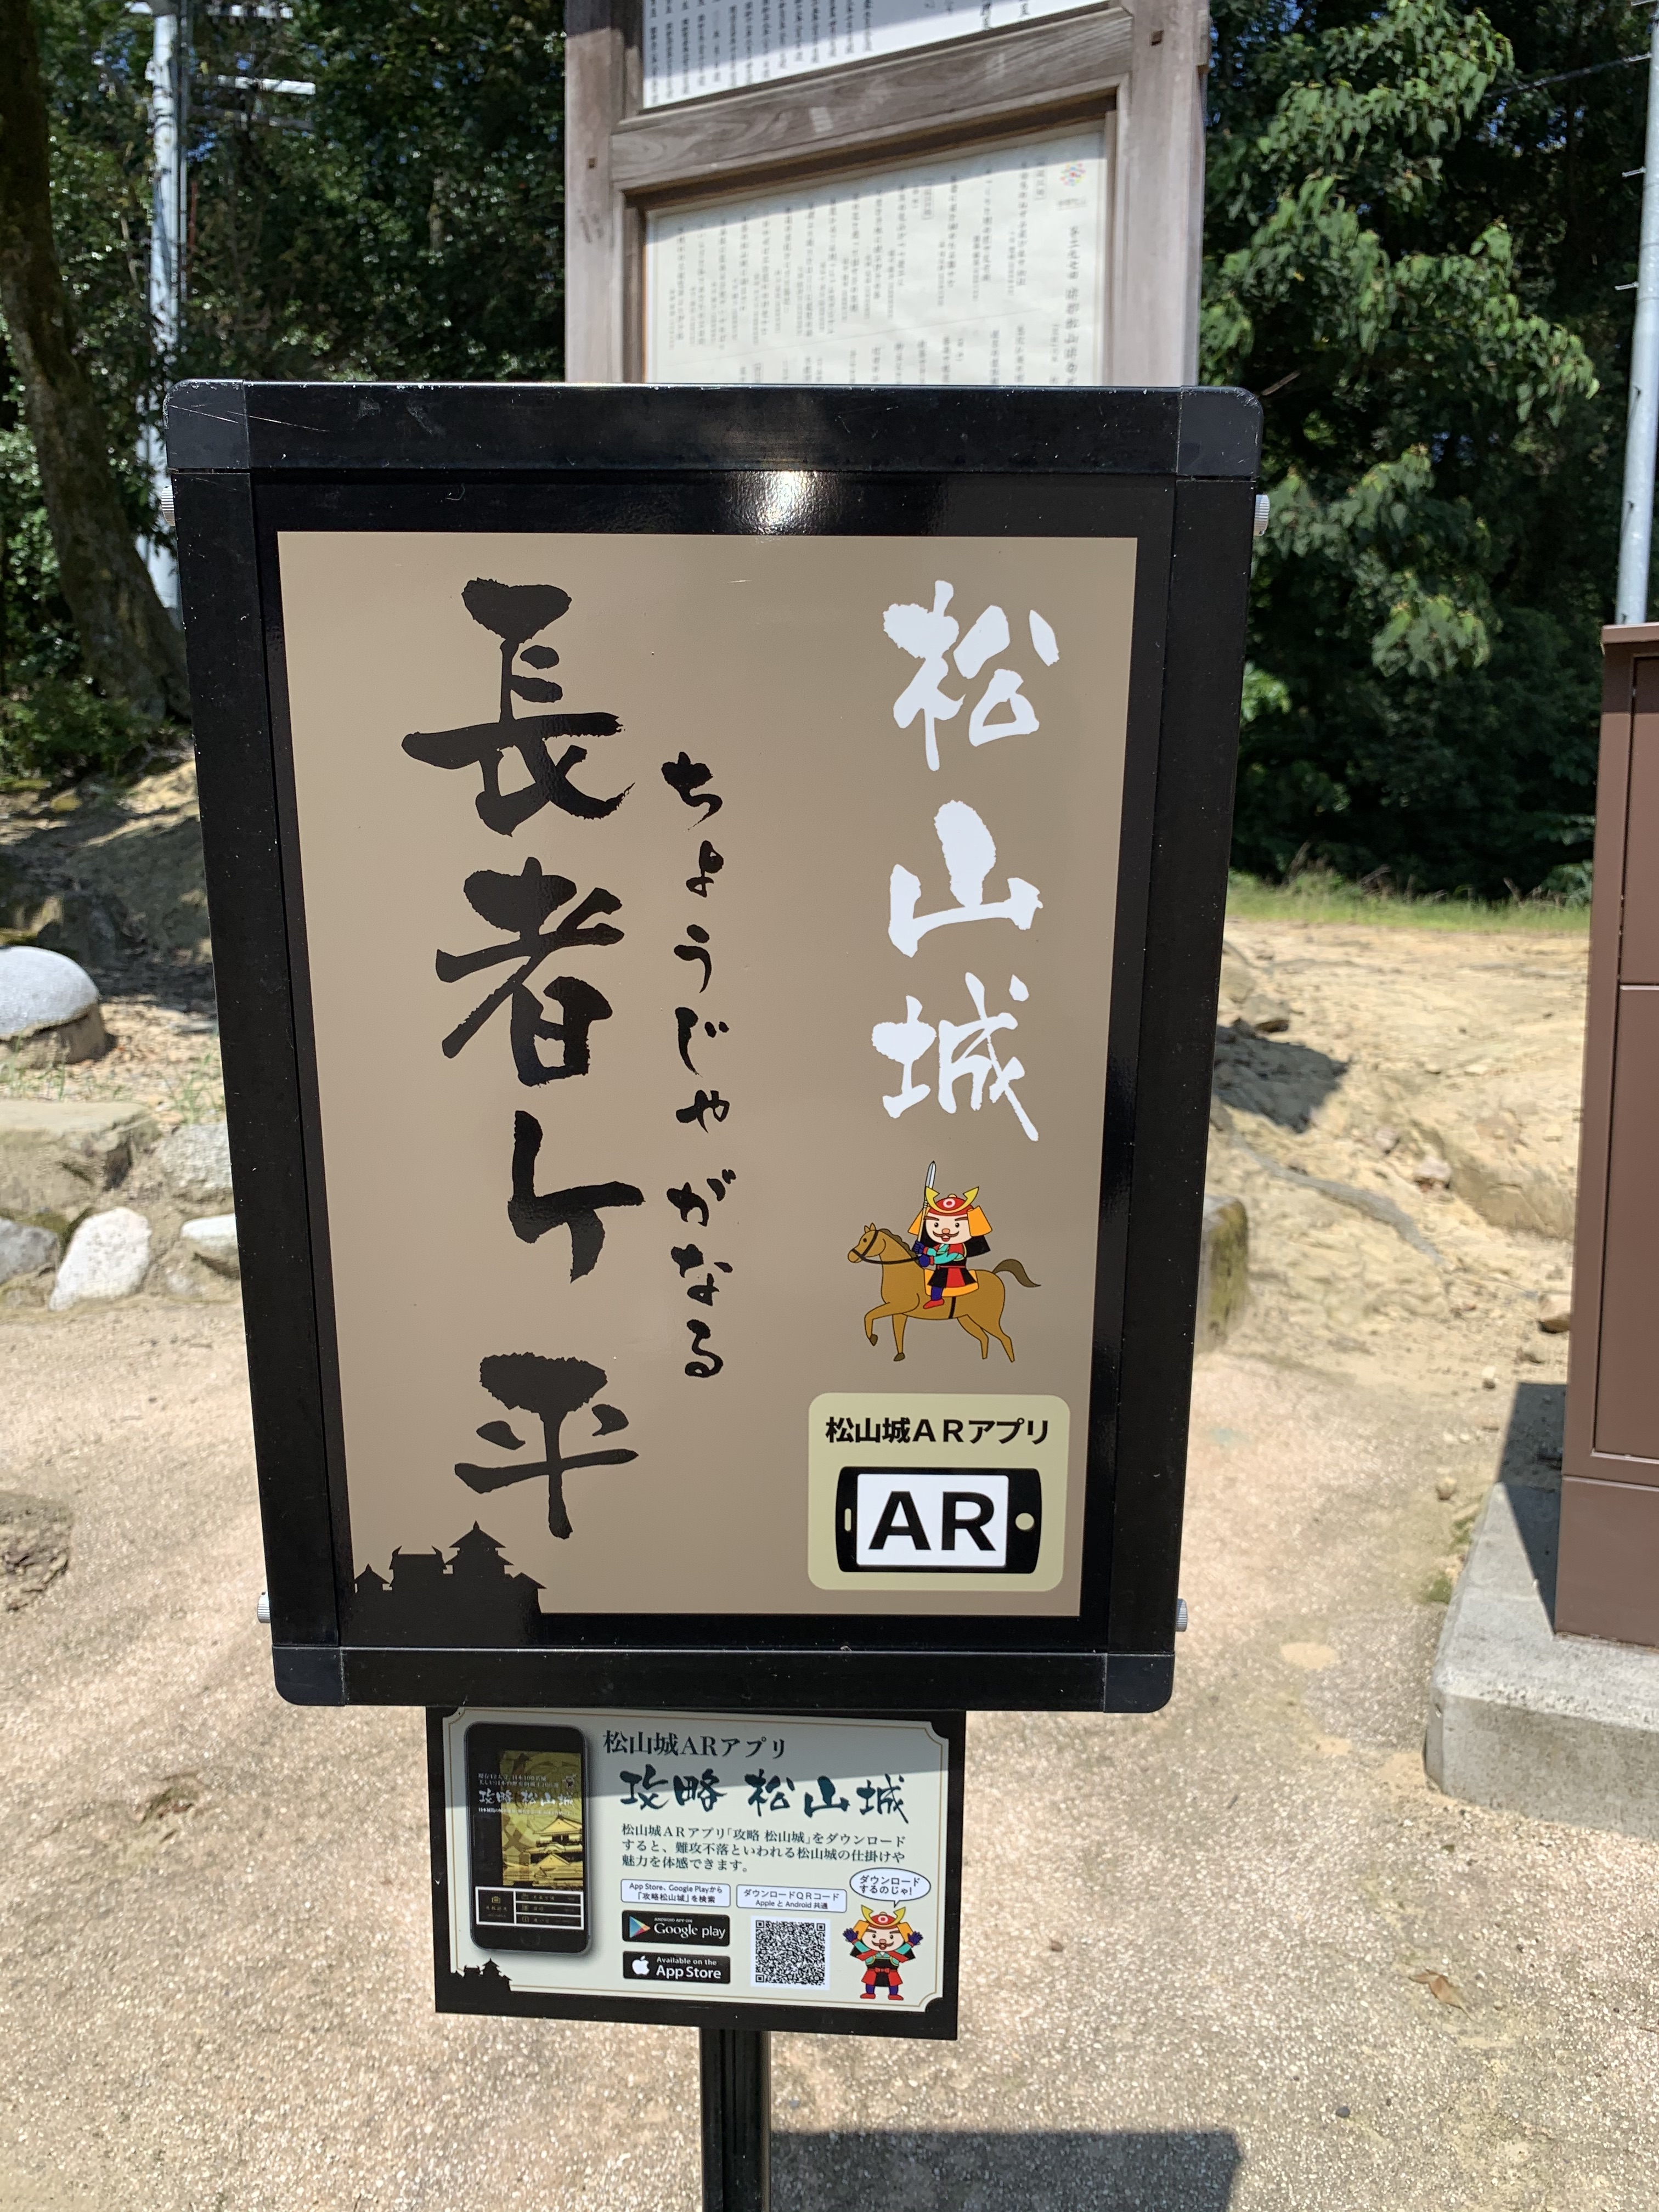
\includegraphics[width=70mm]{images/matsuyama_marker.jpg}
    \caption{専用のマーカー} \label{fig:matsuyama_marker}
  \end{minipage}
  \begin{minipage}{0.5\hsize}
    \centering
    \includegraphics[height=100mm]{images/matsuyama_ar.png}
    \caption{ARでの案内} \label{fig:matsuyama_ar}
  \end{minipage}
\end{figure}



\section{ARによるナビゲーションの問題点}
\label{problems}
前節で述べた現状を元に既存のARによるナビゲーションシステムの問題点を整理する。
ARのナビゲーションシステムには以下のような問題点がある。

\begin{itemize}
  \item 立ち上げるまでのインタラクションが面倒\\
    前節の「遺跡・史跡のARナビゲーションアプリ」のようにマーカーベースのARナビゲーションでは(1)設置されたマーカーを元にアプリを選択、(2)アプリを起動、(3)カメラでマーカーを中心に収めるという3ステップが必要になる。
    GPSと方位情報から位置測位を行うアプリケーションの場合、このような手順は必要ないが後述するように精度が悪く用途か限られるという問題がある。
  \item 位置測位の方法によって精度や用途が大きく限られる\\
    ARでのナビゲーションを行う際に多く用いられる位置測位の方法は、(1)マーカーを使う方法と(2)GPSによる座標検知と方位情報をあわせて利用する方法の2通りに大別される。
    (1)の場合マーカーが読み込めれば精度は高いが、ある程度の距離からカメラで十分認識できるサイズのマーカーを設置する必要がある。
    (2)の場合特別な設備は必要ないが精度面に疑問が残ることに加え、GPS電波の届く屋外に利用が限定される。
    前節で挙げたGoogleMapのAR機能ではGPSや方位情報に加えGoogleが撮影した道路の画像を元に補正を行い、精度を上げているが周囲の景色が登録されていない屋内での利用ができないという問題点は残る。
  \item 情報の登録・編集が面倒\\
    ARで単に目的地の位置を表示したり、決め打ったデータを表示するARナビゲーションアプリは多いが、情報の登録や編集の簡易さに焦点を置いた物は少ない。
    一方でARで表示したい情報は常に変化する可能性があり、今後も増加していくことが予想される。
    このような状況で一般ユーザが気軽に情報を登録編集できる環境を整えることは非常に重要である。
  \item 関連情報を参照・管理することができていない\\
    ARでの表示する情報が増えるにしたがってそれらを互いに参照したり、ドメインごとに管理するニーズは高まっていく。
    しかしながら既存のナビゲーションアプリではARで表示した情報同士を互いに参照して関連情報を表示したり、特定の分野でや条件でフィルターすることが難しい。
  \item 汎用性のあるアプリケーションがない\\
    上記のように「情報の登録・編集が面倒」、「関連情報を参照・管理することができていない」という問題点から特定の目的や分野に限ったARナビゲーションアプリは存在するものの、分野や目的を横断した汎用的ARナビゲーションアプリは開発されていない。
    そのため現状では目的や施設ごとにアプリケーションをユーザ側で切り替える必要があり、ARナビゲーションアプリが増えるほどユーザの負担は大きくなる。
    ユーザの目的やニーズは多岐に渡るためニーズごとにアプリケーションを分けて推薦するのではなく、様々な種類の情報を包括的に管理できるシステムが求められている。
    さらに目的や施設ごとにアプリケーションと情報が独立してしまうことで分野を横断したつながりを表現できないという問題点も生まれる。
\end{itemize}



\section{テキストや画像の進化}
前節で述べたとおりARによるナビゲーションには課題が多いが、ナビゲーションに利用しているテキストや画像などのメディアは計算機の進化とともに発展し、多くの問題点を克服している。

計算機上で利用されているテキストは、文字から内容を検索することが可能なため文書の参照や管理が格段に行いやすく、あらゆる文書が電子化されたテキストに置き換えられるようになった。
またWebやハイパーリンク等の技術によってより参照しやすくなったほか、別の文書を引用する等の再利用が可能になった。
さらにハイパーリンクを含んだ文書を手軽に作成・編集できるWiki\cite{Leuf2001TheWW}が登場したことでより柔軟で活発なテキストによる知見の共有や情報の再利用が実現された。

同様に画像や地図などのメディアも電子化とWebの進歩により参照や管理が格段に行いやすくなった。
SNSや画像の管理が行えるクラウドウェアの普及により誰しもが写真を撮影し容易にWeb上にアップロード/公開することが可能になった。
このようにして公開された画像はURLによって一意に参照することができ、画像の再利用性は大きく高まった。
またGoogle Mapsのように、地理情報システム(GIS : Geographic Information System)が誰でも検索・参照可能な形でWebに公開されることで位置情報や地理情報を参照することが容易になった。

このような文書以外のメディアの進化に合わせ、近年の文書作成システムやWikiシステムは画像/音声/動画/地図といったマルチメディアを自在に埋め込む機能を持っている。

\section{Wikiとナビゲーションへの利用}
\subsection{Wiki}
WikiはWard Cunninghamが提案した不特定多数のユーザーが文書コンテンツを編集・管理するためのWebシステムである。
Wikiには以下のような特徴があり、情報を集積するコンテンツで多く活用される。
\begin{itemize}
  \item ブラウザを使って誰でもWeb上で情報編集/共有ができる、
  \item 文書間にリンクが張りやすく、個々の文書が高度に連携した文書群を作成しやすい
\end{itemize}

\subsection{現状のナビゲーションの限界}
第\ref{current}節で挙げたとおり現状のナビゲーションシステムは決まった目的地へ案内することを目的とする物が多い。
また目的地の検索機能を有していても、ユーザは能動的にキーワードを入力し目的地を絞り込む必要がある。
一方で、ナビゲーションを必要としているユーザの多くは漠然と達成したいことがあっても実際の目的地が分かっていない。
場合によっては達成したいこと自体が曖昧で言語化できていないこともある。
このような場合、ユーザに目的地を指定・検索させて案内をする現状のナビゲーションではユーザの目的を達成する事ができない。
ユーザ側に目的に関する知識や明確な意思がない場合に案内をできないことが現状のナビゲーションの限界であると言える。

\subsection{Wikiの有用性}
上記のようなナビゲーションの限界を解決するために必要な要素は以下であると考える。
\begin{enumerate}
  \item 幅広い分野の情報を提示することができる
  \item ユーザが周囲の情報を能動的に探索できる
  \item その結果自身の目的を明確化し目的地を確定できる。
\end{enumerate}
このような要素は情報管理ツールとしてWikiを利用すること満たすことができる。
Wikiは情報を分野で階層化・グルーピングすることなく一元的に管理する。
そのため1のように分野にとらわれない情報の提示が可能である。
またWikiはハイパーリンクによって文書間で参照しており、関連情報へのアクセスが容易である。
この特徴によって2のようにリンクをたどりながら自分の興味のある分野へページを遷移し、情報を探索することができる。
さらに探索によってユーザは周囲の情報を知識として吸収し、3のように目的を明確化することができる。
以上のような理由からナビゲーションにWikiを利用することで既存のナビゲーションの限界を打破した新しい形のナビゲーションが提供できると考える。


\section{NFC技術とインタラクション}
ARでのナビゲーションシステムには自身の位置情報やその場のコンテキスト情報が不可欠であり、一般的にそのような情報を瞬時に取得することは難しい。
一方NFCタグには以下のような特徴があり、実世界においてその場のコンテキスト情報や設置された物の情報を記述するのに便利である。

\begin{itemize}
  \item 電源がいらない
  \item 非常に薄く、小型
  \item IDやURLなどを記録するには十分な記憶容量を持つ
  \item 一枚あたり10円前後と安価
\end{itemize}

近年では多くのモバイル端末にNFCタグの読み取り機能が搭載されており、一般的なNFCタグであれば誰でも書き込まれた情報を瞬時に読み取ることができる。
さらに書き込むデータ形式によっては、モバイル端末でNFCタグの読み取るだけでWebページを開いたり、アプリを起動することが可能である。

このようなNFCタグの特徴は、現在一般的な用途である決済や在庫管理、家電操作などに加えナビゲーションシステムを補助するシステムとして有効であると考える。

一方でNFCタグは読み取る際に、読み取る機器をNFCタグにかなり近づける必要があるという制約がある。
この技術的制約は一般的にデメリットとして捉えられがちであるが、NFCタグを読み取ったタイミングでのユーザの持つ端末の位置はNFCタグとほぼ接していると確定できるとも言える。
つまりNFCタグに位置情報をもたせることができれば非常に小さい誤差でユーザの持つ端末をの位置を確定できることになる。
この特徴は第\ref{problems}節で述べた問題点の1つであるNFCの位置測位の問題を解決する。





\section{まとめ}
ARをナビゲーションとして利用するアイデアは以前から存在し、モバイル端末の普及と発展により実用段階に来ているプロダクトも増えている。
しかしながら第\ref{problems}節に上げた問題点を解決できていないため、汎用的なヘルプ・ナビゲーションとして利用されるに至っていない。
一方でナビゲーションに利用しているテキストや画像などのメディアは計算機上で積極的に応用されており、ハイパーリンクやWiki等の技術によって参照や再利用がより行いやすくなった。
また近年多くのモバイル端末に搭載されているNFC技術には第\ref{problems}節であげた問題点の一部を克服する可能性がある。
したがってARの正確な位置測位とコンテキスト情報の取得にNFCの技術を利用しつつ、ARで表示する情報の管理にWikiの手法を取り入れることで第\ref{problems}節に挙げた問題を解決できると考える。
次章では第\ref{problems}節に挙げたARナビゲーションシステムが持つ問題点を解決した、次世代のARナビゲーションシステム「HypAR Touch」を提案する。  % 本文2
\chapter{設計}
\label{chap:design}

本章では次世代のARナビゲーションシステム「HypAR Touch」の要件と設計について述べる。

\newpage

\section{要件}
前章で整理したARナビゲーションシステムの問題点を踏まえた上でHypAR Touchシステムの要件を整理する。
\begin{enumerate}
  \item 手軽なインタラクションでアプリケーションの起動と位置測位ができる。
  \item 周囲のコンテキストを簡単に指定できる。
  \item ARでの表示情報を容易に登録・編集できる。
  \item ハイパーリンクを利用し、関連情報を参照・管理することができる。
\end{enumerate}
これらの要件を満たすARナビゲーションシステムは、NFCをタッチするインタラクションとハイパーテキストの編集環境であるWikiの組み合わせによって実現できる。

\section{設計}
NFCを利用したインタラクションとWikiを採用することで前節に上げた要件を満たすことを説明し、本システムの設計を記述する。

\subsection{NFC技術の利用}
前章で述べた通りNFCタグの持つ様々な性質はナビゲーションシステムにとって有用である。
この性質を利用し、NFCタグのタッチからアプリの起動と位置測位を行うことで前節の要件1を満たすことができる。
またNFCタグに記録された情報から周囲のコンテキストを把握することで前節の要件2が達成される。

\subsubsection*{要件1:手軽なインタラクションでアプリケーションの起動と位置測位ができる}
NFCタグによるインタラクションにはカメラでマーカーを読み込むインタラクションなどと比べて以下のような優位性がある。
\begin{itemize}
  \item データの読み込みが非常に早い
  \item モバイル端末でアプリが起動していない状態でも読み込み可能である
  \item 周囲の明るさなどの環境要因に左右されず安定して読み込み可能である
\end{itemize}
このようなNFCタグによるインタラクションの特徴を利用し、HypAR Touchでは次のような動作を設計した。
\begin{enumerate}
  \item NFCタグに緯度経度・方位の情報を記録する。
  \item NFCタグへのタッチを契機にアプリケーションを起動する。
  \item NFCタグを読み取るには数センチ以内の距離で平行にタッチする必要があるため、モバイル端末の位置が確定する。
  \item 3での前提を元にNFCタグに記録された緯度経度・方位の情報から初期位置を算出する。
  \item アプリの起動後は4で設定した初期位置とモバイル端末の加速度センサによるデータを組み合わせ位置を算出する.
\end{enumerate}
これにより「NFCタグにタッチする」という手軽なインタラクションでアプリケーションの起動及び位置測位が実現できたことになる。

\subsubsection*{要件2:周囲のコンテキストを簡単に指定できる}
NFCタグには上記の特徴以外にも以下のような利点がある。
\begin{itemize}
  \item 小型である
  \item 電源がいらない
  \item 情報を埋め込める十分な容量
\end{itemize}
このような特徴は実世界に設置し周囲のコンテキスト情報を記録する媒体として非常に優れている。
本研究においてはNFCタグを利用し、緯度経度情報や方位の情報のみならず設置している物や場所に合わせた情報なども記録する。
また本システムは普及に向けた観点から、事業者やユーザーなどシステムに詳しくない一般人がタグを設置するを想定している。
そのためNFCタグを利用することには上記の理由に加え以下のような点からもメリットがある。
\begin{itemize}
  \item 1枚あたりのコストが十数円と非常に安価である
  \item 読み込み距離を担保できれば外見を気にすることがなく設置が楽である
\end{itemize}
本システムではこのような特徴を活かし、誰もがNFCタグを設置できるよう一意なIDを記録したNFCタグを配布し、
貼り付けた場所の情報をアプリから登録する方法を採用した。


\subsection{Wikiの利用}
Wikiはハイパーリンクを含んだ文書を手軽に作成・編集・管理できるツールである。
WikiシステムをAR情報の管理・編集ツールとして利用することで前節の要件3、4を満たすことができる。

\subsubsection*{要件3:ハイパーリンクを利用し関連情報を参照・管理することができる}
Wikiはハイパーリンクによってページ間にリンクを張ることができ、個々のページが高度に連携した文書群を作成することができる。
その結果適切にリンクが貼られていれば文書内のリンクを辿るだけで容易に関連情報を参照することが可能である。
このようなWikiの特徴はナビゲーションシステムにおける関連情報の提示に適しているといえる。

\subsubsection*{要件4:ARでの表示情報を容易に登録・編集できる}
現在多く使われるWikiシステムにはWeb上で内容を編集する仕組みが標準で備わっており、誰もが容易に内容を登録・編集することが可能である。
またハイパーリンクやタグの記述に加え、画像や動画といったメディアの参照・埋め込み機能に対応しているシステムも多い。
このように高機能な編集機能をもったWikiをARナビゲーションの情報源として利用することでAR情報を容易に登録・編集できる環境を実現する。

\begin{figure}[H]
  \centering
  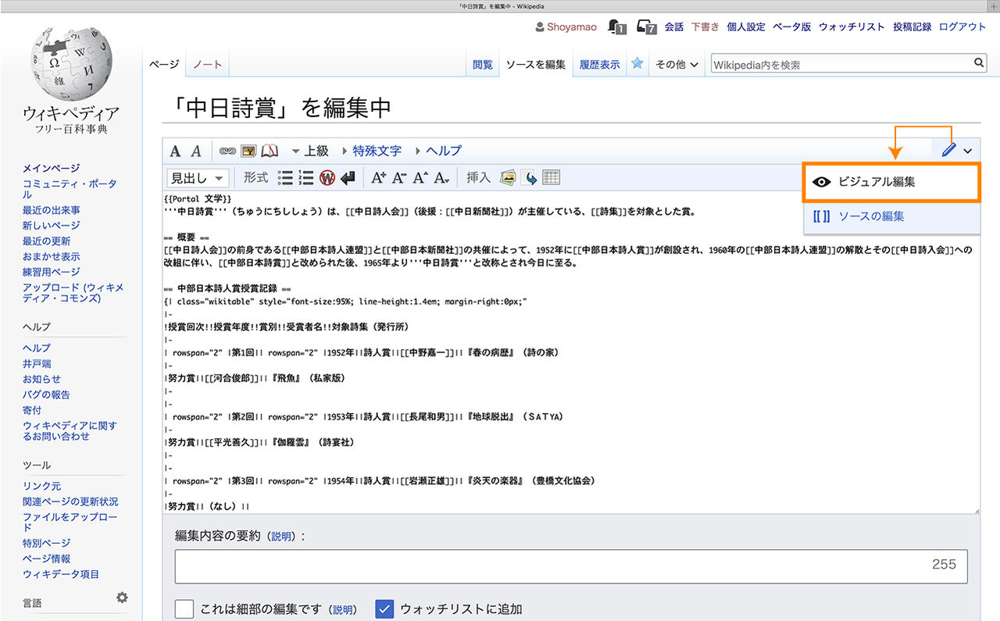
\includegraphics[width=120mm]{images/wikipedia_edit.png}
  \caption{Wikipediaでの編集画面} \label{fig:wikipedia_edit}
\end{figure}

\subsection{NFC技術とWikiの併用}
上記のようなNFC技術とWikiの利点を組み合わせることで前節の要件5も満たすことができる。

\subsubsection*{要件5:広い分野の知見と用途を総合的に管理できる}
Wikiはハイパーリンクで情報を整理・参照するため、グループによる情報分類や階層的な情報の管理を必要としない。
したがってWikiでは異なる分野の情報をフラットに管理し、参照することができる。
実際ににWikiシステムを利用した百科事典であるWikipediaはあらゆる分野の情報を総合的に管理しながらも破綻なくシステムを運用している。
このようなWikiシステムをAR情報の管理に利用することで、分野を横断した知見の管理が可能になり、様々な用途に対応したナビゲーションシステムを作成できる。

Wikiシステムを利用すると広い分野の情報を一元的に管理することができるが、一方で自身の欲しい情報を探す際に手間となる事がある。
これを避けるためにNFCタグに記録されたコンテキスト情報を活用し検索・フィルタが可能なシステムを本研究では採用した。

これより広い分野の情報を一元的に管理できるWikiの利点を活かしながら様々な用途に対応したナビゲーションを提供する事が可能となる.



\section{まとめ}
本章では第\ref{chap:background}章で整理したARナビゲーションの現状と問題点を元に次世代ARナビゲーションシステム、HypAR Touchの要件を定義した。
さらに定義した要件はNFC技術とWikiシステムを組み合わせることで達成されることを提案し、その詳細を設計で示した。
次章では本設計を元に開発したHypAR Touchの実装とその機能を説明する。  % 本文3
\chapter{実装}
\label{chap:implementation}

本章では第\ref{chap:design}章で述べたシステムの設計を元にした、HypAR Touchの実装及び機能について述べる。

\newpage

\section{アプリケーション構成}
HypAR TouchはARナビゲーションを表示するモバイルアプリケーション、AR情報やNFC情報を永続化しAPIを提供するサーバー、Scrapbox、Gyazo\footnote{\textsf{https://gyazo.com}}、NFCタグで構成される(図 \ref{fig:application_structure})。

\begin{figure}[H]
  \centering
  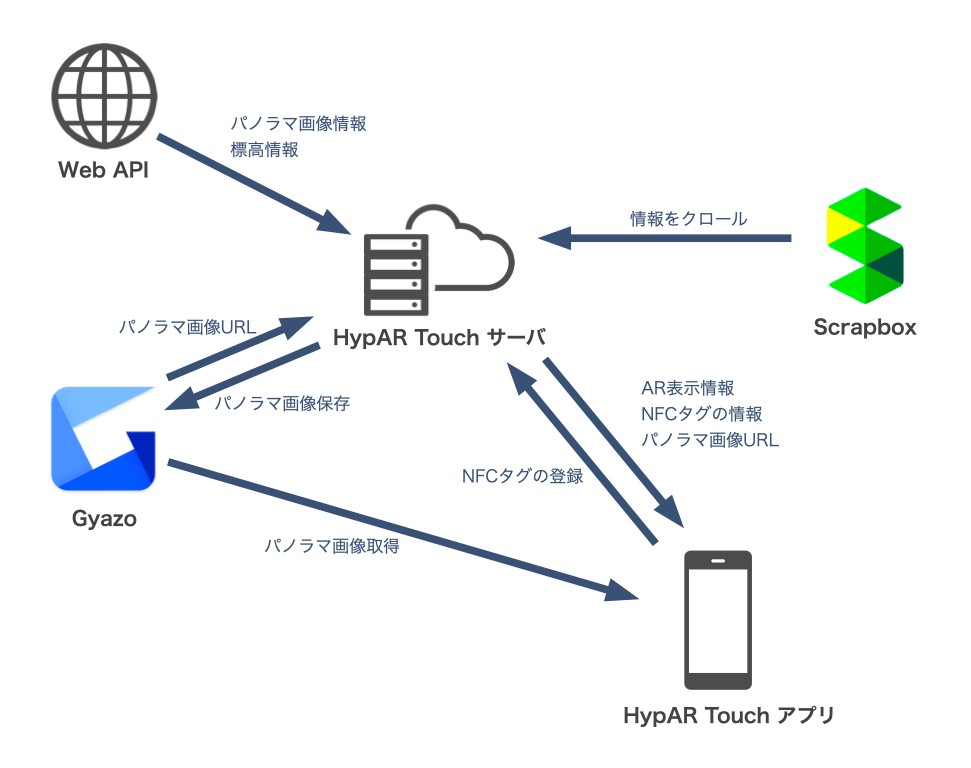
\includegraphics[width=150mm]{images/application_structure.jpg}
  \caption{構成図} \label{fig:application_structure}
\end{figure}

\subsection{Scrapbox}
Scrapbox(図\ref{fig:scrapbox})はGyazz\cite{Gyazz}をベースにして開発された、Nota\footnote{\textsf{https://www.notainc.com/ja}}社が運営しているWikiである。
本システムではこのScrapboxをARで表示する情報の管理ツールとして利用している。
これはScrapboxが他のシステムには存在しない以下のようなHypAR Touchに適した特徴を持つためである。
\begin{itemize}
  \item シンプルで柔軟な記法をもつWYSIWYGエディタ
  
  入力/改行/段落/箇条書きといった基本的なテキスト編集を見たまま行える。
  
  \item 場所指定に最適なLocation記法
  
  Google MapsのURLを貼り付けるだけで地図を埋め込めるLocation記法\footnote{\textsf{https://scrapbox.io/help-jp/Location記法}}と呼ばれる機能があり地理情報を記述するのに適している。
  本システムではこのLocation記法によって表示する情報の場所を指定している。

  \item リンク記法によるシンプルなハイパーリンクと関連ページリスト
  
  Scrapboxでは単語を\texttt{[]}で囲うだけで同一Wiki内ページへのリンクとすることが可能である。
  さらにScrapboxページの下部には
  \begin{itemize}
      \item 別ページへのリンク
      \item 別ページからのリンク
      \item リンク先ページがリンクしているページ
  \end{itemize}
  といった関連ページリスト(図\ref{fig:scrapbox_related})が表示され、どのような情報と関連するのかが一目瞭然に分かる。
\end{itemize}

\begin{figure}[H]
  \begin{minipage}{0.5\hsize}
    \centering
    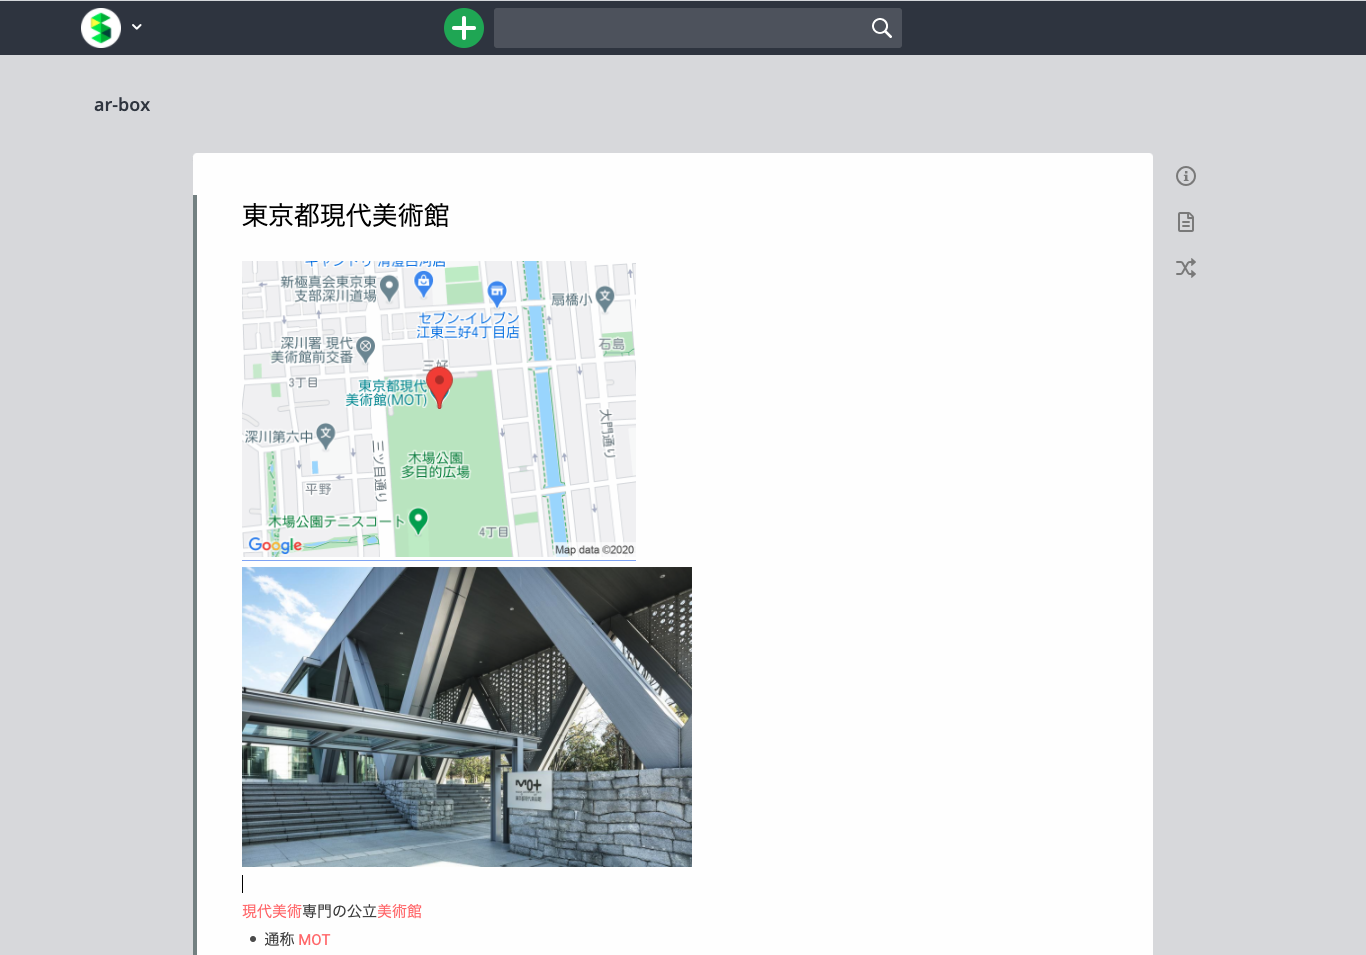
\includegraphics[width=75mm]{images/scrapbox_screen.png}
    \caption{Scrapboxの画面} \label{fig:scrapbox}
  \end{minipage}
  \begin{minipage}{0.5\hsize}
    \centering
    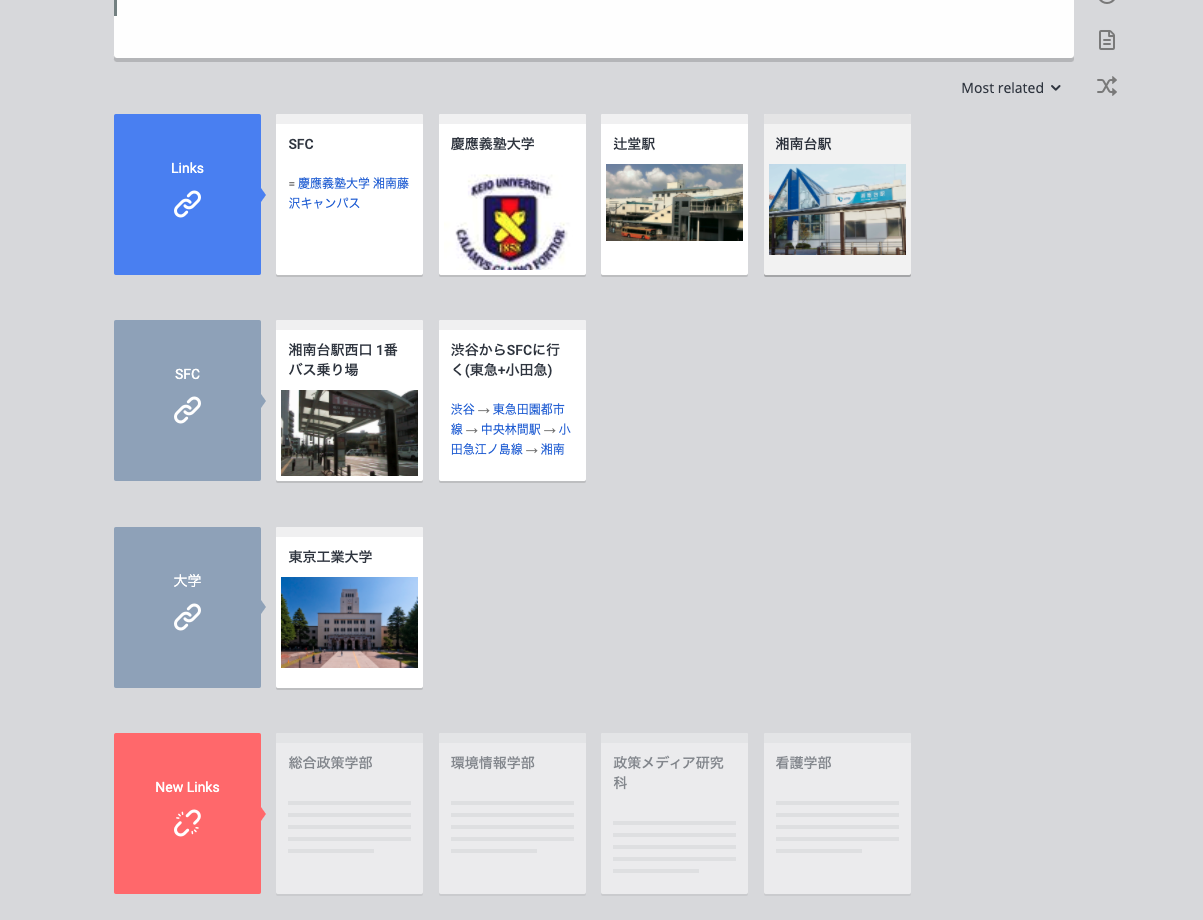
\includegraphics[width=75mm]{images/scrapbox_related_screen.png}
    \caption{Scrapboxの関連ページリスト} \label{fig:scrapbox_related}
  \end{minipage}
\end{figure}

Scrapboxでは文書の集合であるWikiを「プロジェクト」という単位で管理しており、プロジェクトによってメンバ・公開設定等を設定可能である。
プロジェクト内のページはすべてフラットに管理され、上記の記法でページ間をハイパーリンクでつなぎ容易に参照できる。
HypAR TouchではNFCタグで対象とするScrapboxのプロジェクトを選択できるようにしている。
またHypAR Touchではプロジェクト内の1ページがARで表示される1つのノード対応するようなっている。

Scrapboxはプロジェクト内のページリストと各ページの情報を取得するAPI\footnote{\textsf{https://scrapbox.io/help-jp/API}}を持っており、これを利用することでHypAR TouchサーバはScrapboxをクロールしている。


\subsection{HypAR Touchアプリ}
HypAR TouchアプリはReactNative\footnote{\textsf{https://reactnative.dev/}}と呼ばれるフレームワークを利用して作成されたモバイル端末アプリケーションである。
ReactNativeはWeb技術を利用し、マルチプラットフォームなモバイル端末向けアプリケーションを作成するためのフレームワークである。
このReactNative利用することでHypAR TouchアプリはAndroidとiOSの両方に対応したアプリケーションとなっている。

HypAr TouchアプリはNFCに記録された一意なidを取得し、そのidに紐付いた以下の情報を後述するHypAr Touchサーバーから取得する。
\begin{itemize}
  \item NFCタグの緯度経度
  \item NFCタグの設置される向き(0〜360度)
  \item 表示するAR情報の元となるScrapboxのプロジェクト名
  \item タッチした時に選択されているリンク情報
\end{itemize}
さらに取得したScrapboxのプロジェクト名をもとにHypAR TouchサーバーからARで表示する情報を取得する。
その上で取得したARの情報とNFCタグの緯度経度、NFCタグの設置された向きをもとに、各AR情報の位置を相対的に算出している。
また各AR情報には登録された位置付近で撮影されたパノラマ画像のURLが含まれている。
視点移動機能ではこのURLで登録された360度画像からVRのビューを作成している。

\subsection{HypAR Touchサーバ}
HypAR TouchサーバはNode.js\footnote{\textsf{https://nodejs.org/}}上で動作するWebアプリケーションとして実装されている。
HTTPリクエストを処理するWebアプリケーションフレームワークとしてExpress\footnote{\textsf{https://expressjs.com/}}を用い、
そのホスティング環境としてBaaS(Backend-as-a-Service)の1つであるHeroku\footnote{\textsf{https://www.heroku.com/}}を利用している。
HypAR TouchサーバはHypAR Touchアプリで利用するAR情報やNFCタグ情報を管理する役割をもっており、その機能は大きく4つに分けられる。

\begin{itemize}
  \item 対象となるScrapboxのプロジェクトをクロールし、AR表示に必要な情報を整理した上で永続化する。\\
  HypAR Touchサーバは指定されたScrapboxのプロジェクトを定期的にクロールし、位置情報やサムネイル画像のURL、リンク情報など、AR表示に必要な情報をまとめてデータベースに永続化している。
  これによりユーザがScrapboxに加えた変更がARでの表示に対応するようになっている。
  \\
  \item 登録されたNFCタグに関する情報を永続化する。\\
  NFCタグには一意なidが記録されており、それに紐づく形でタグの位置情報や向き、対象とするScrapboxプロジェクトなどの情報がこのサーバーに記録される。
  \\
  \item クロールした情報を元にパノラマ画像を生成し、Gyazoに保存した上でそのURLを記録する。\\
  第3章で記述した視点移動機能を実装するためにはARで表示する情報に加えて、記録された位置情報に最も近いところから撮影されたパノラマ画像が必要である。
  そのためHypAR TouchサーバではARで表示する情報ごとにGoogle Street ViewのAPI\footnote{\textsf{https://developers.google.com/maps/documentation/streetview/overview}}を利用してその地点からのパノラマ画像を生成している。
  また、画像の保存・永続化には後述するGyazoを利用しており、最終的にはGyazoに保存されたパノラマ画像のURLをARで表示する情報と合わせてデータベースに永続化している。
  \\
  \item 上記3つの情報を取得・追加・変更するAPIを提供する。\\
  HypAR Touchサーバは上記3つの情報を生成・永続化するだけでなく、HypAR TouchアプリからのAR情報取得やNFCタグの登録を受け付ける必要がある。
  そのためHypAR Touchサーバはこれらの情報を取得、追加、更新するAPIを提供している。

\end{itemize}


\subsection{Gyazo}
Gyazoは、パソコンのデスクトップ画面の一部をキャプチャしてWebにアップロードするツールおよび画像を保存する画像/映像専用のクラウドストレージサービスである。
Gyazoには十分な保存容量があり、画像のアップロード・取得等のAPIも揃っている。
そのため自身のサーバよりも安全に画像を管理可能なGyazoを本システムでのパノラマ画像の保存先として利用している。

\subsection{NFCタグ}
本システムで利用するNFCタグはモバイル端末のOSに関わらず、読み込めるタグ形式とデータフォーマットでなくてはならない。
そのため本システムではNFCタグとして最も普及しているISO/IEC 14443 TypeAに準拠したNFCタグを利用している。
また同様にNFC FORUMが策定したデータフォーマットであるNDEFを利用することでNFC機能を持つほとんどのモバイル端末に対応している。
NDEFのデータ形式には更に細かく、Text、URI、SmartPostermの3つのタイプが存在する。
このうちURIタイプで書かれたNFCタグは殆どのNFC対応スマートフォンでのバックグラウンド読み取りに対応している。
またAndroidとiOSにはディープリンクと呼ばれる特殊なURIからインストールされたアプリケーションを起動する機能が存在しており、そのURIの形式をCustom URL Schemeと呼ぶ。
Custom URL Schemeでは図\ref{fig:custom_url_scheme}のように起動するアプリの指定だけでなく、URIパラメータを利用して追加の情報を記述しアプリケーション側にその情報を渡すことが可能である。
このような特徴を踏まえ、本システムではNFCタグにCustom URL Schemeの形にしたURIをNDEFのURIタイプとして記録している。
これにより、モバイル端末でNFCタグにタッチするだけでアプリの起動及びタグIDの受け渡しが可能となる。

\begin{figure}[H]
  \centering
  
\includegraphics[width=150mm]{images/custom_url_scheme.jpg}
  \caption{Custom URL Scheme} \label{fig:custom_url_scheme}
\end{figure}




\section{機能}

\subsubsection{HypAR Touchアプリによるナビゲーション閲覧}
\paragraph*{NFCタグにタッチする}
本アプリケーションは図\ref{fig:touch_nfc}のように専用の情報が書かれたNFCタグにタッチすることで起動し、ナビゲーションを開始する。
NFCにタッチすることで端末の位置と向きが認識され、図\ref{fig:hypar_touch_init_screen}のように登録された情報をARで正しい位置に表示することができる。
また画面下部にあるスライダー(図\ref{fig:hypar_touch_slider})を動かすことでARで表示する情報の距離の範囲を指定することができる。

\begin{figure}[H]
  \centering
  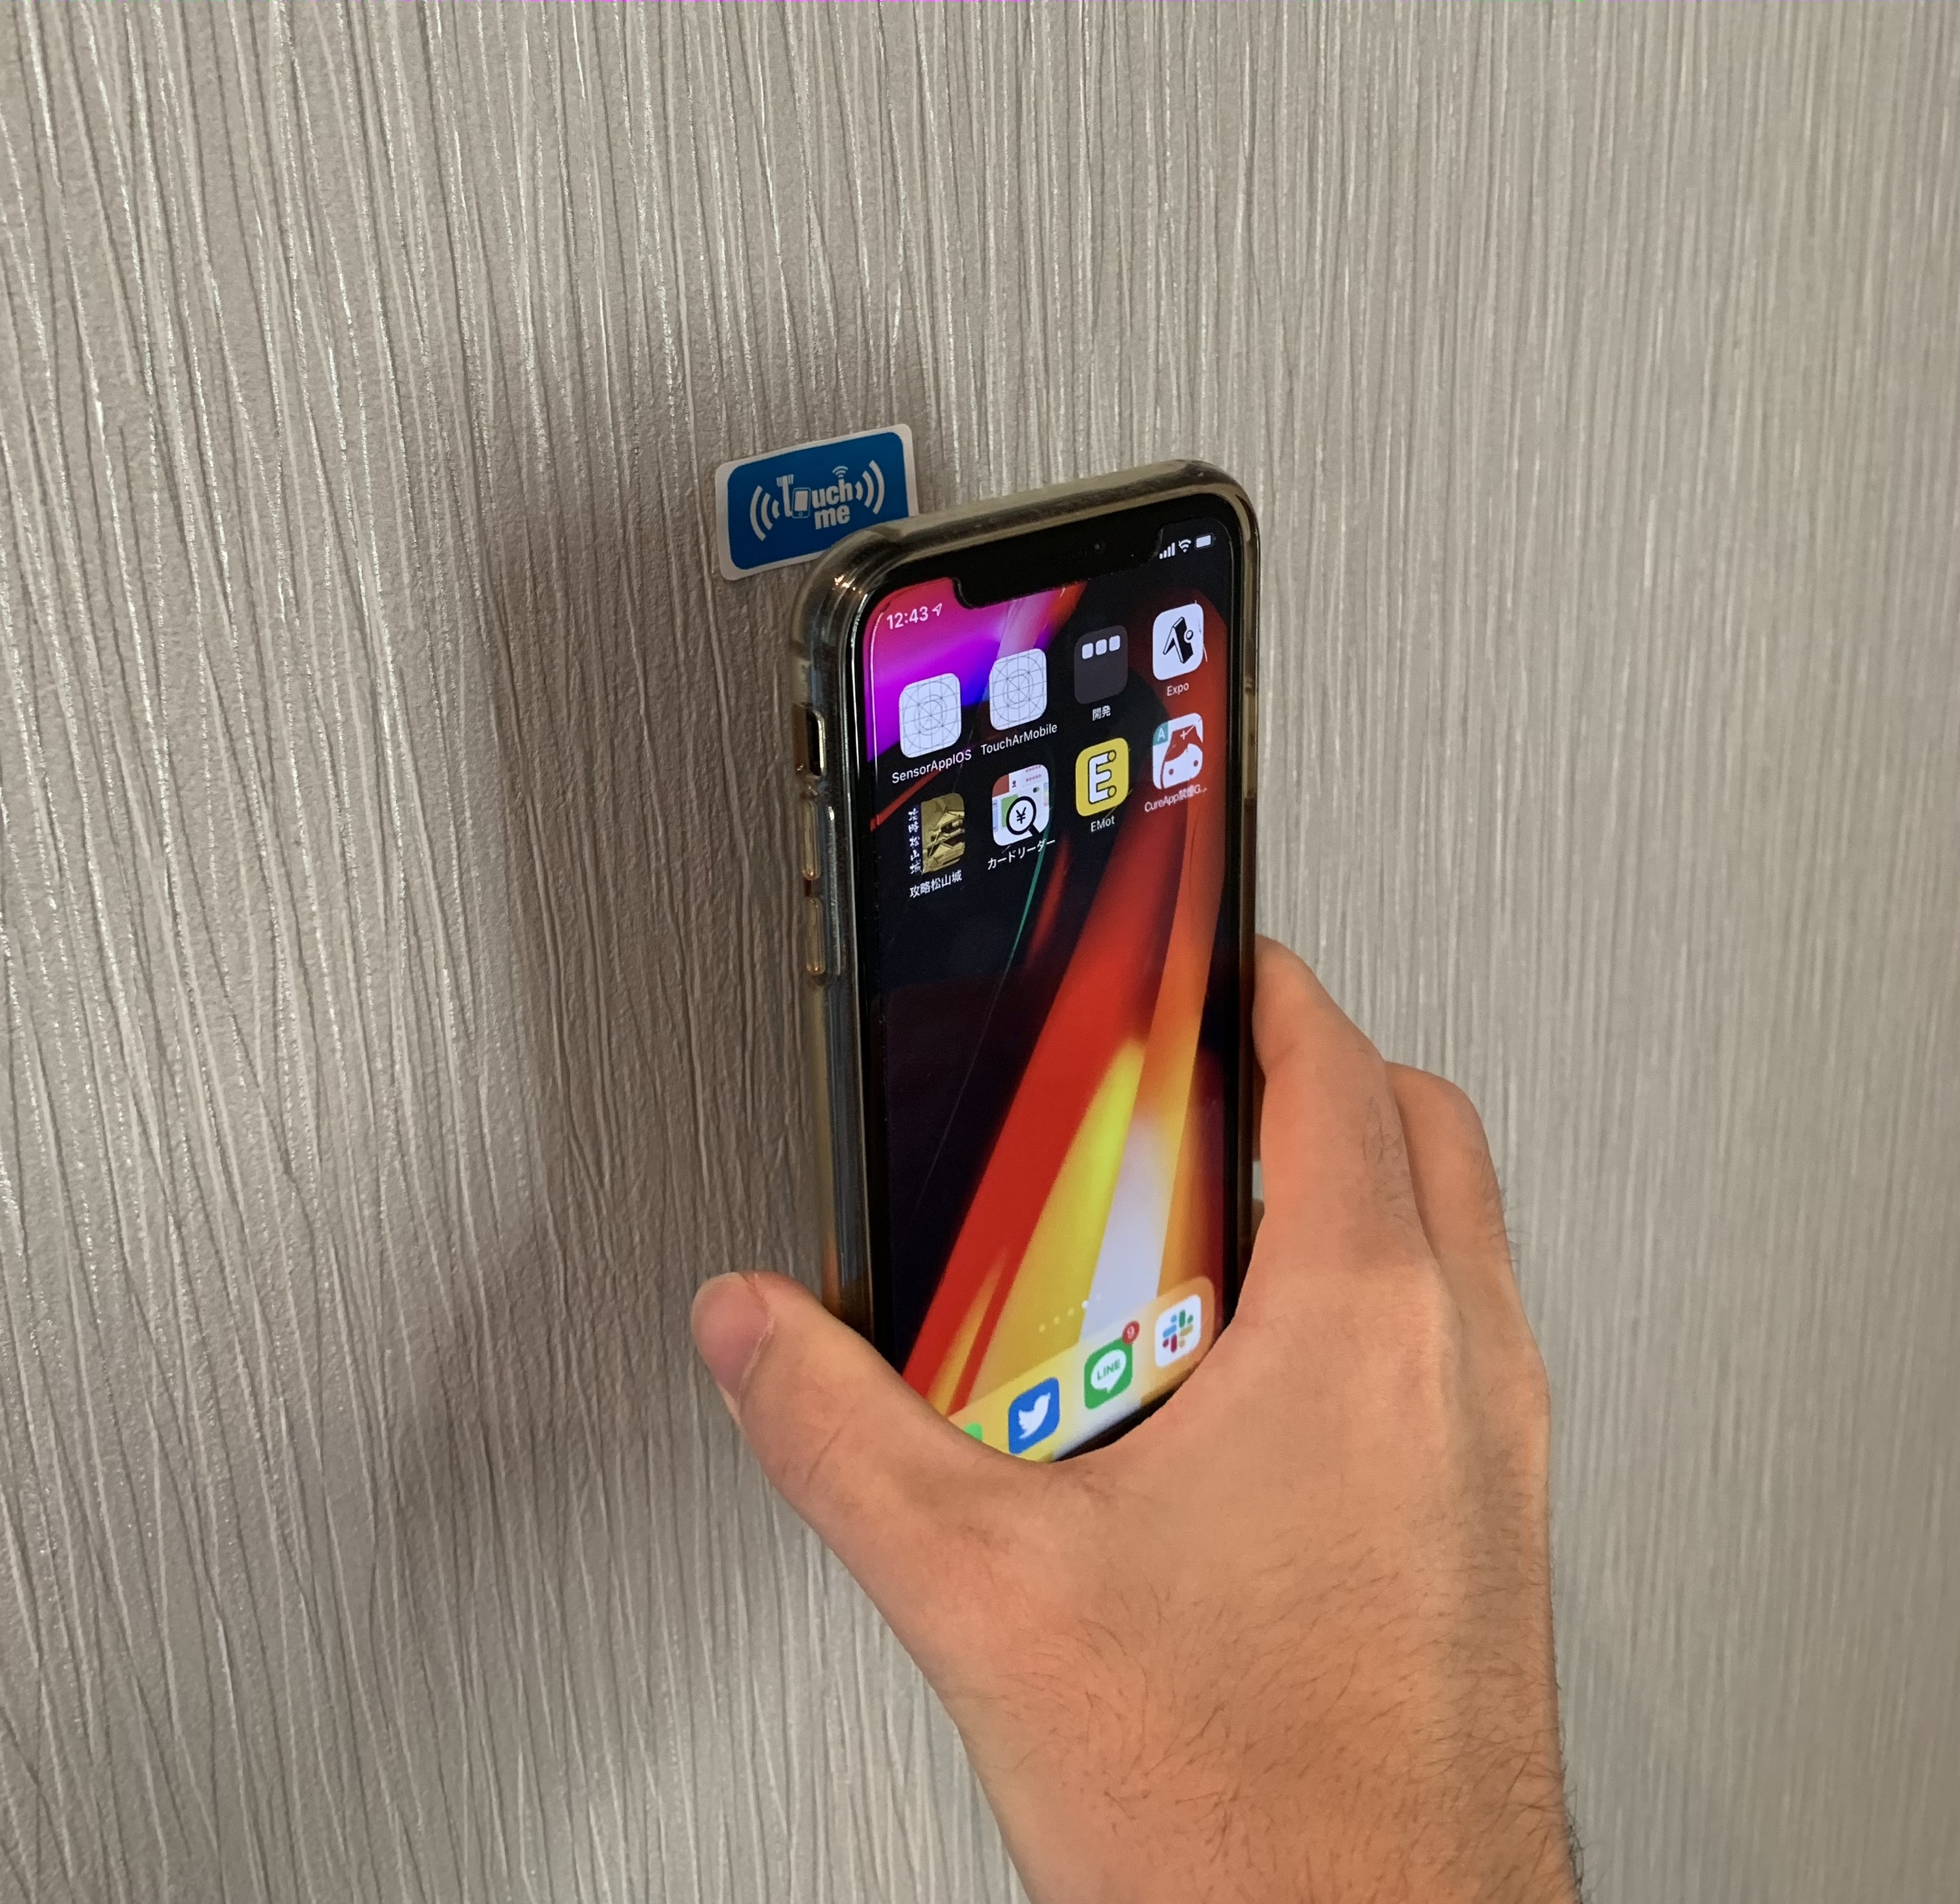
\includegraphics[width=100mm]{images/touch_nfc.jpg}
  \caption{NFCタグにタッチする様子} \label{fig:touch_nfc}
\end{figure}

\begin{figure}[H]
  \begin{minipage}{0.5\hsize}
    \centering
    \includegraphics[height=100mm]{images/hypar_touch_init_screen.png}
    \caption{ARでの表示} \label{fig:hypar_touch_init_screen}
  \end{minipage}
  \begin{minipage}{0.5\hsize}
    \centering
    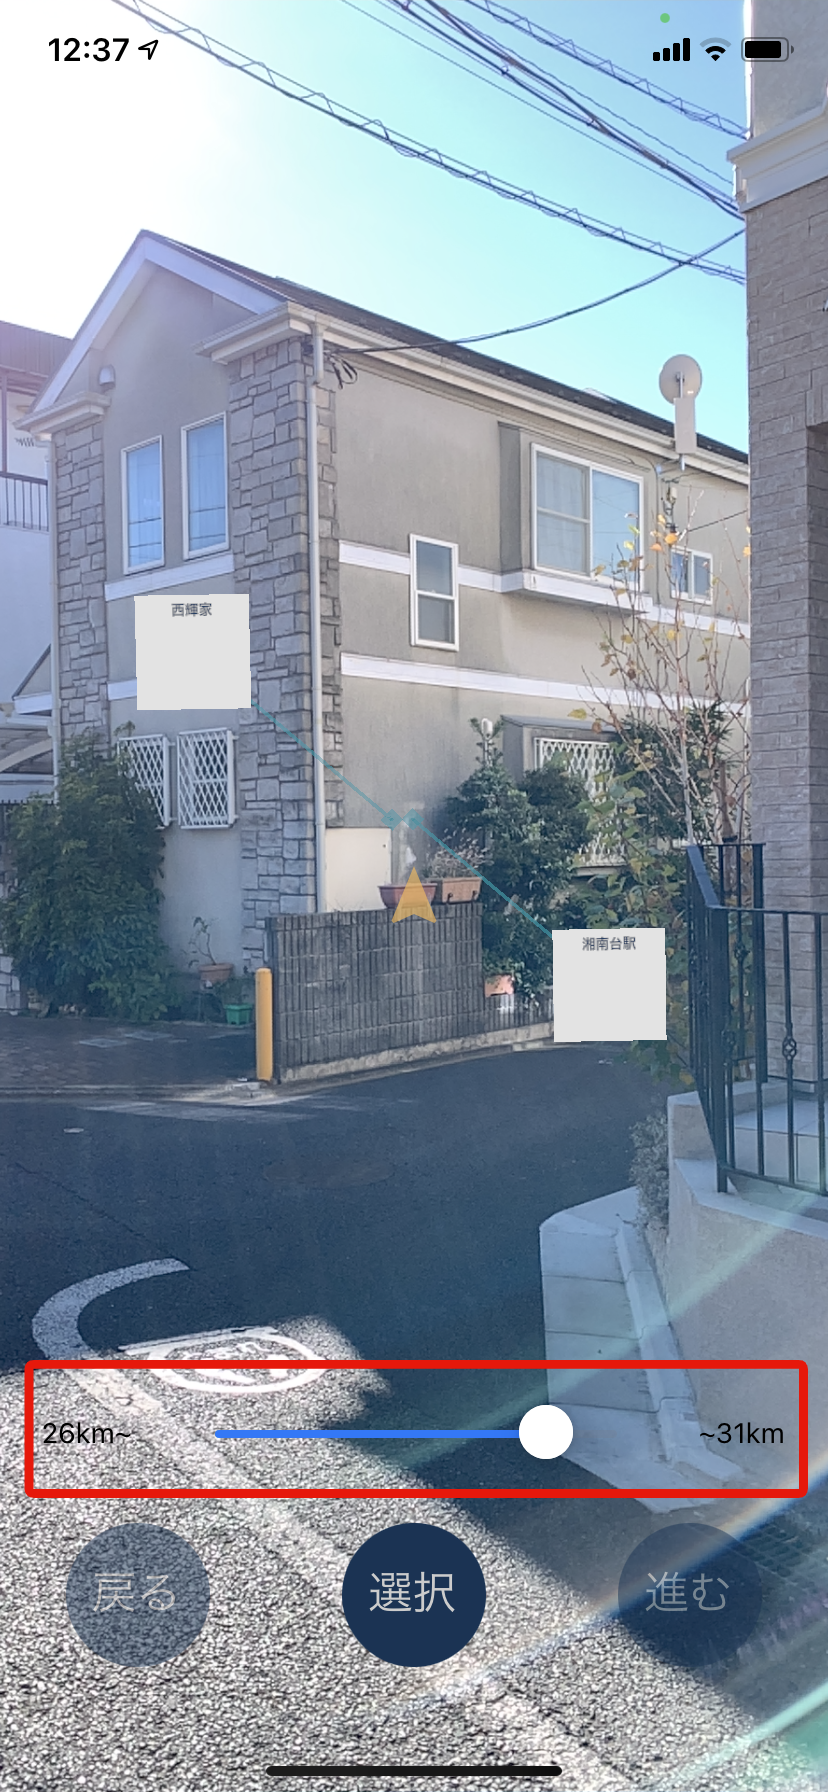
\includegraphics[height=100mm]{images/hypar_touch_slider.png}
    \caption{スライダーによる距離指定} \label{fig:hypar_touch_slider}
  \end{minipage}
\end{figure}

\paragraph*{表示されたAR情報の関連情報を表示・選択する}
画面の中央にはオレンジ色の三角のカーソルが表示されており、これをARで表示された情報の上に重ねると青い枠線が表示される(図\ref{fig:hypar_touch_hover})。
その状態で画面下部の選択ボタンを押すと図\ref{fig:hypar_touch_selected}のように関連する情報が放射状に配置されてに表示される。
これらの表示された関連情報も同じようにカーソルで選択することができる(図\ref{fig:hypar_touch_sub_selected})。
このように関連情報を選択していくことによって興味のある情報をAR上で探索することができる。

\begin{figure}[H]
  \begin{minipage}{0.5\hsize}
    \centering
    \includegraphics[height=100mm]{images/hypar_touch_hover.png}
    \caption{カーソルを重ねた状態} \label{fig:hypar_touch_hover}
  \end{minipage}
  \begin{minipage}{0.5\hsize}
    \centering
    \includegraphics[height=100mm]{images/hypar_touch_selected.png}
    \caption{選択した状態} \label{fig:hypar_touch_selected}
  \end{minipage}
\end{figure}

\begin{figure}[H]
    \centering
    \includegraphics[height=100mm]{images/hypar_touch_sub_selected.png}
    \caption{関連情報の選択} \label{fig:hypar_touch_sub_selected}
\end{figure}


\paragraph*{選択されたAR情報の詳細を見る}
上記のようにカーソルをAR情報にあわせた上で選択ボタンを押すと画面上部には図\ref{fig:hypar_touch_top}のように選択された情報のタイトルの他に「see more」と書かれたボタンが出現する。
これをクリックすることでAR情報の元となったScrapboxをみることが可能である(図\ref{fig:hypar_touch_webview})。

\begin{figure}[H]
  \begin{minipage}{0.5\hsize}
    \centering
    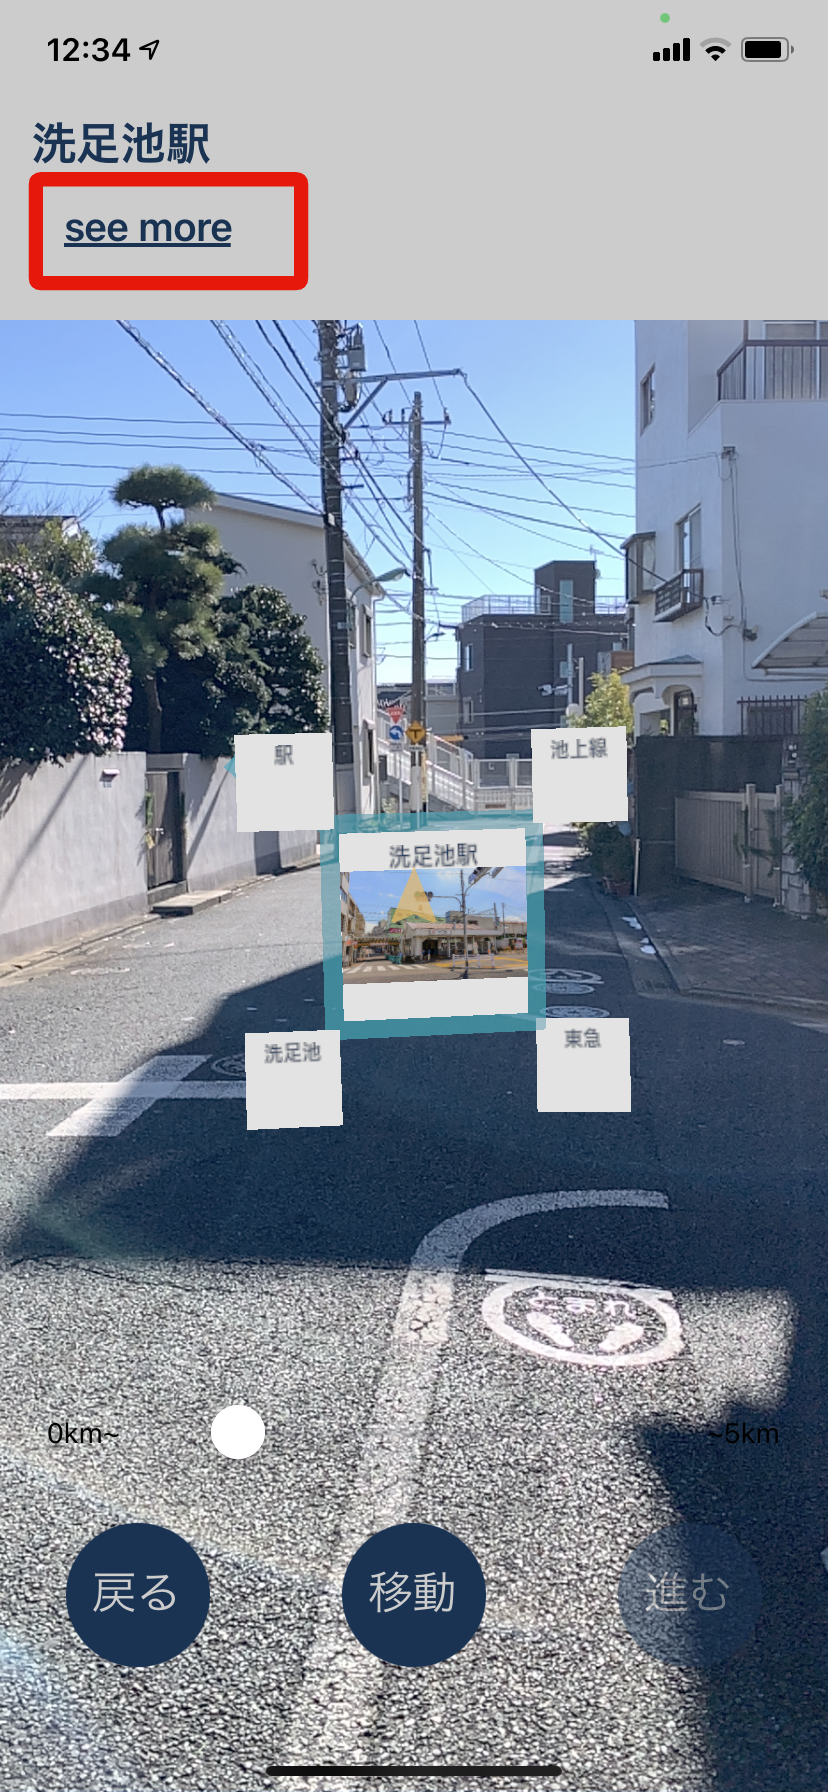
\includegraphics[height=100mm]{images/hypar_touch_top.png}
    \caption{詳細を表示するボタン} \label{fig:hypar_touch_top}
  \end{minipage}
  \begin{minipage}{0.5\hsize}
    \centering
    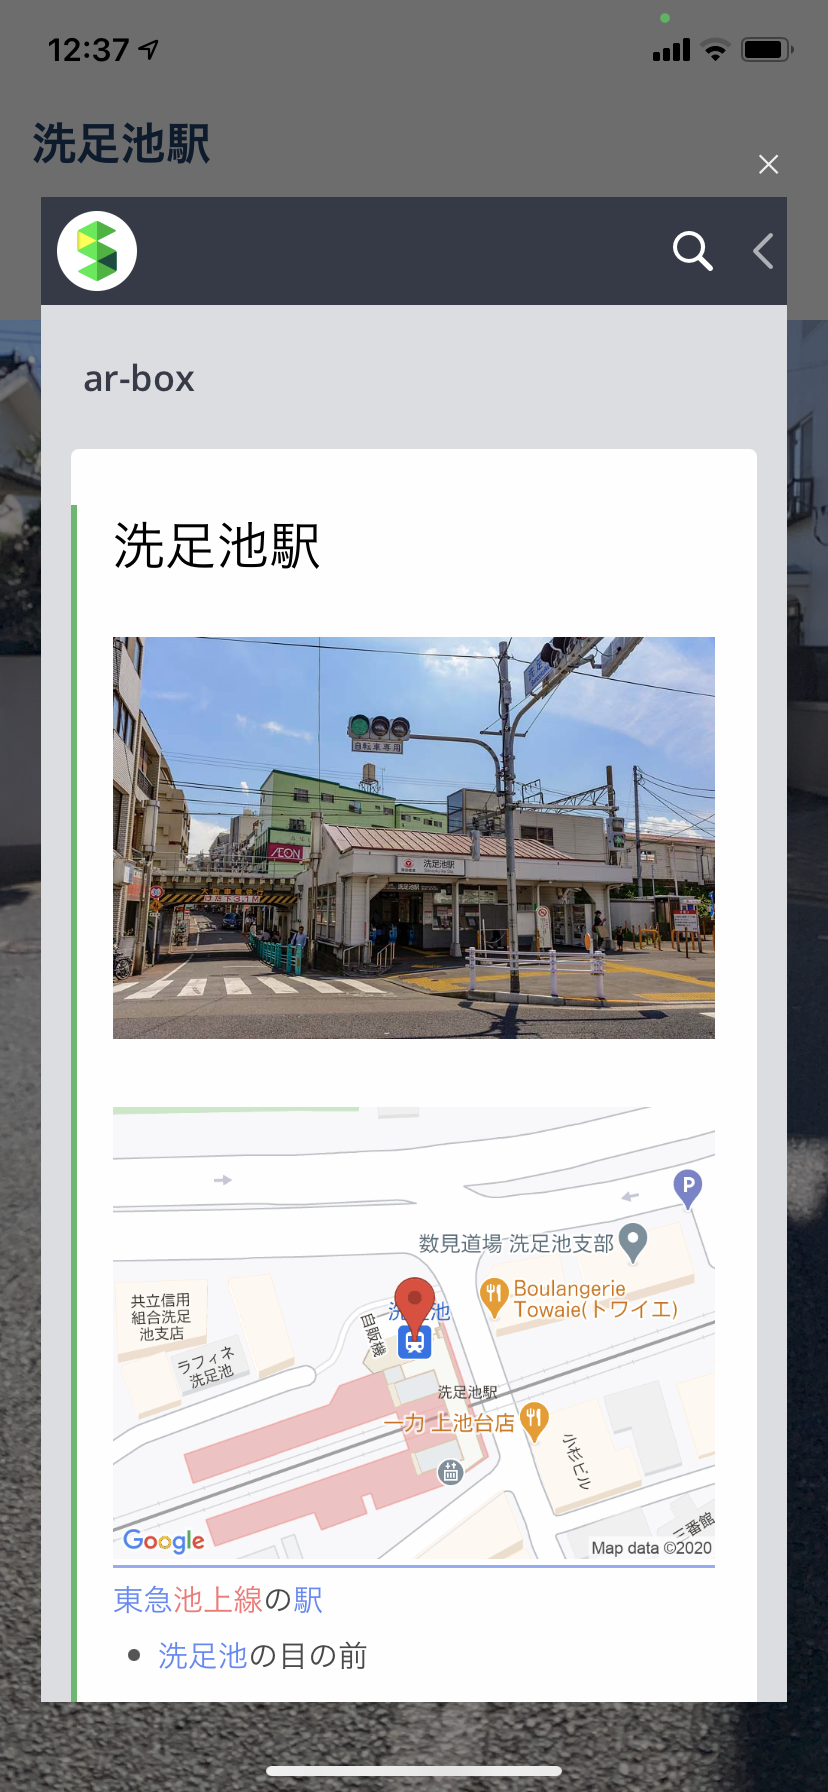
\includegraphics[height=100mm]{images/hypar_touch_webview.png}
    \caption{Scrapboxでの情報表示} \label{fig:hypar_touch_webview}
  \end{minipage}
\end{figure}

\paragraph*{選択されたAR情報の場所に視点を移動する}
同じようにカーソルをAR情報にあわせた上で選択ボタンを押し、もう一度選択したAR情報にカーソルを重ねると画面下部中央のボタンが「移動」に変化する(図\ref{fig:hypar_touch_move_button})
この移動ボタンを押すと図\ref{fig:hypar_touch_move_map}のような地図での移動アニメーションを経て、選択した情報のある場所からの視点(図\ref{fig:hypar_touch_moved})に切り替えることができる。

\begin{figure}[H]
  \begin{minipage}{0.5\hsize}
    \centering
    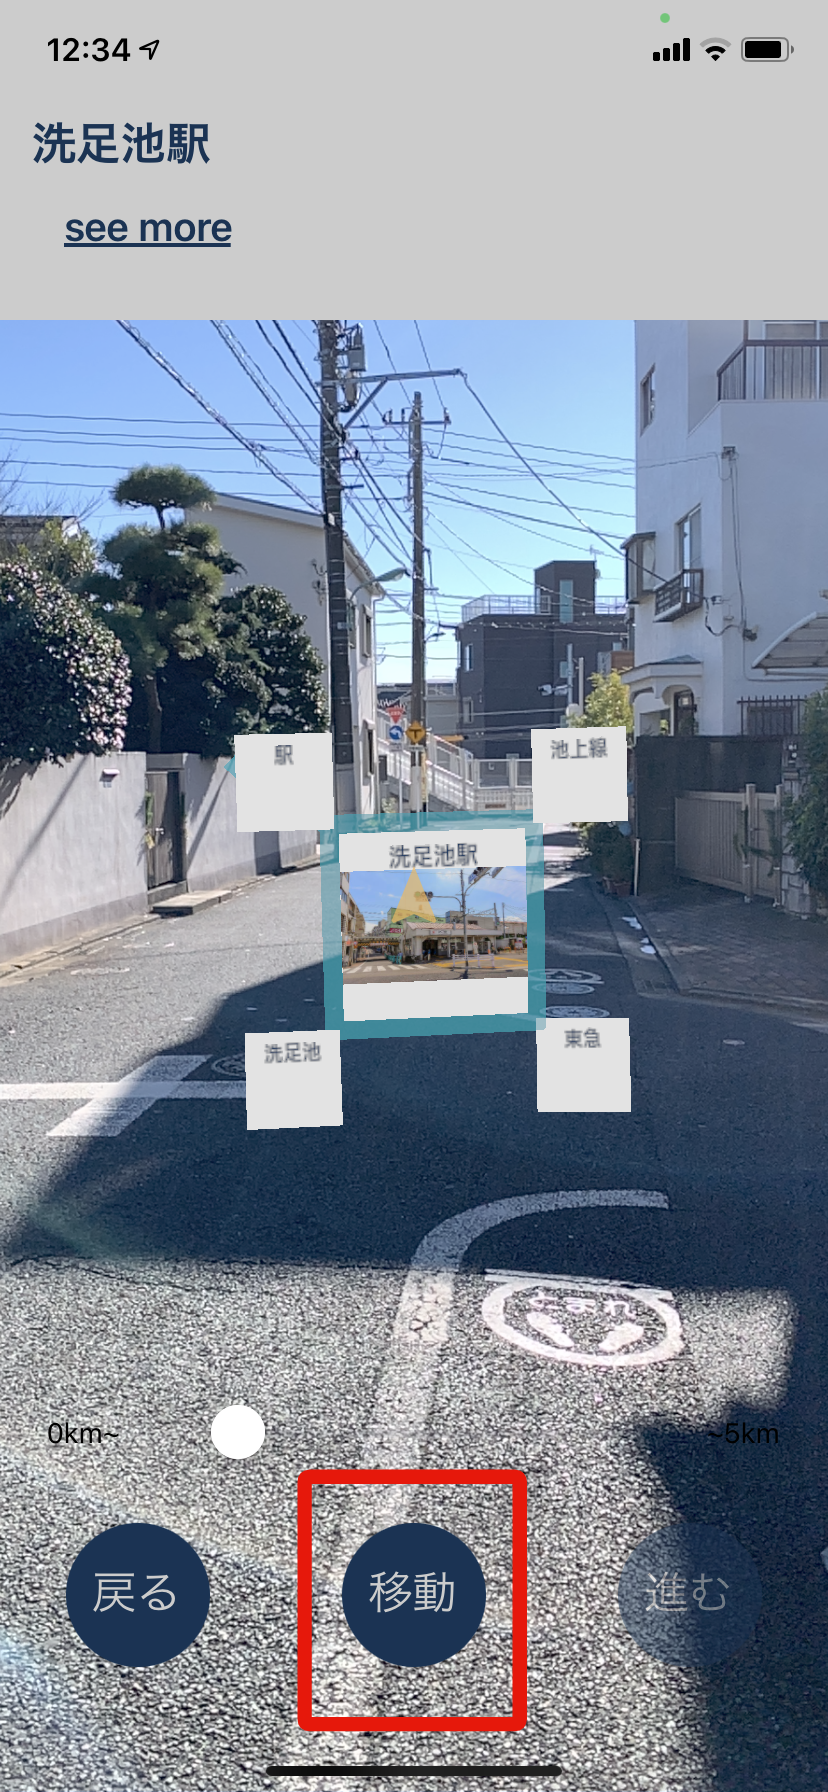
\includegraphics[height=100mm]{images/hypar_touch_move_button.png}
    \caption{移動ボタン} \label{fig:hypar_touch_move_button}
  \end{minipage}
  \begin{minipage}{0.5\hsize}
    \centering
    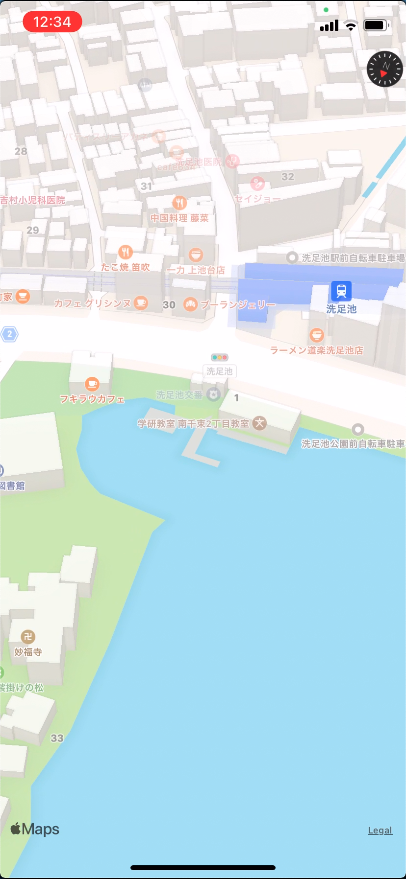
\includegraphics[height=100mm]{images/hypar_touch_move_map.png}
    \caption{Mapでの移動アニメーションの途中} \label{fig:hypar_touch_move_map}
  \end{minipage}
\end{figure}

\begin{figure}[H]
  \centering
  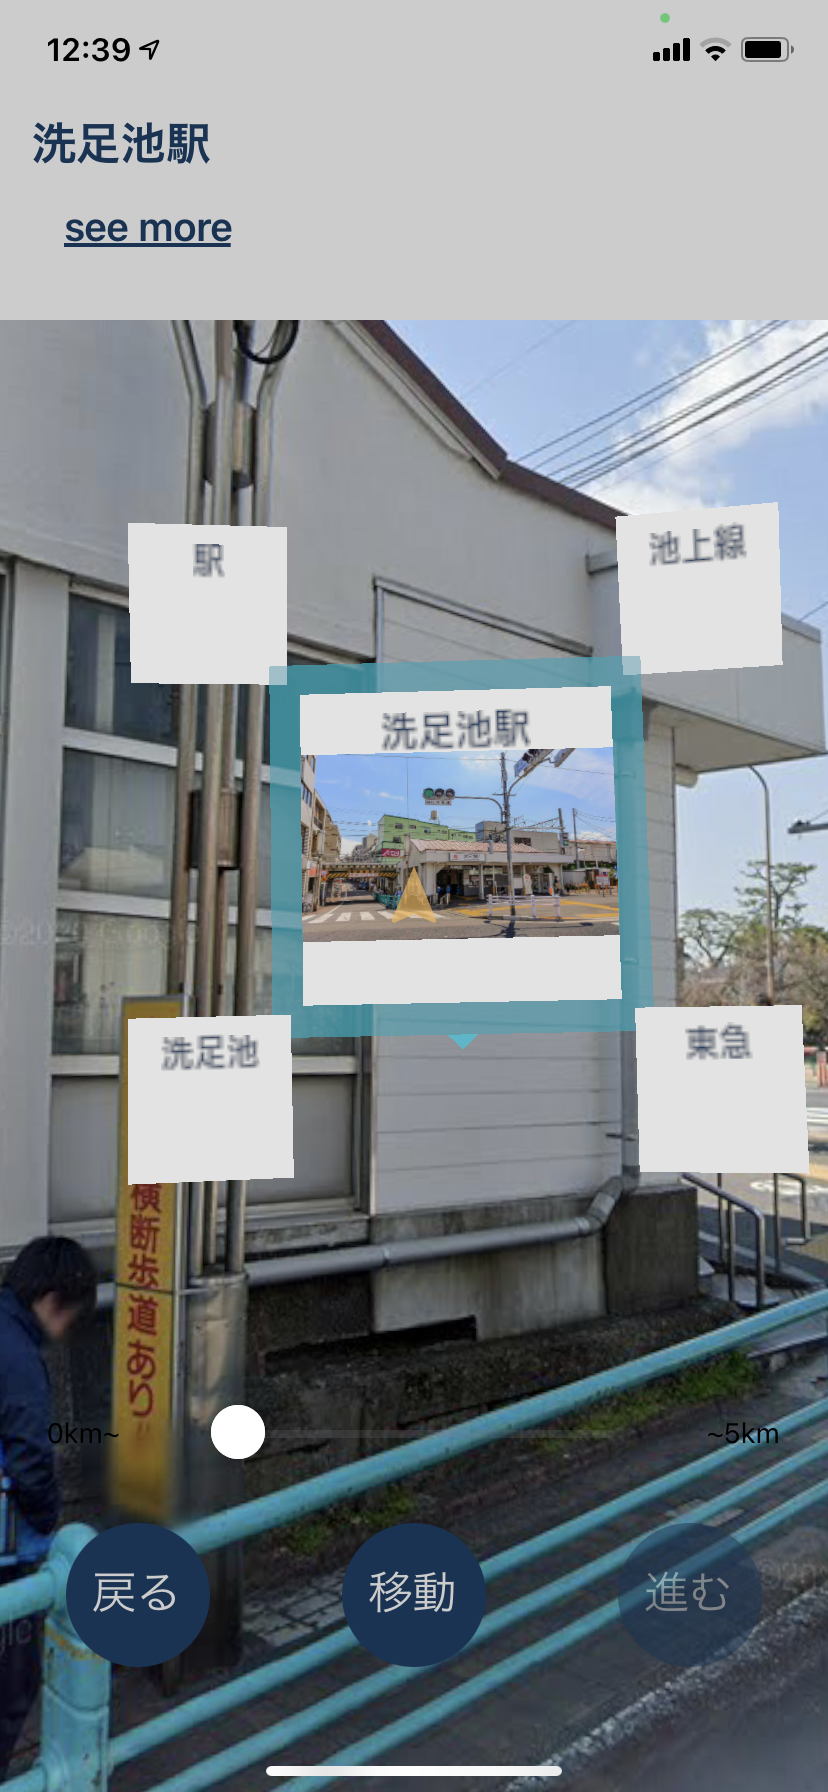
\includegraphics[height=100mm]{images/hypar_touch_moved.png}
  \caption{移動先からの視点} \label{fig:hypar_touch_moved}
\end{figure}

\paragraph*{AR情報の選択を解除する・前の状態に戻る}
上記のような選択状態は画面の何も表示されていない部分をタップすることで解除できる。
また選択や移動した履歴情報は常に保存されており、画面下部の「戻る」「進む」ボタン(図\ref{fig:hypar_touch_history_button})で履歴を参照することができる。

\begin{figure}[H]
  \centering
  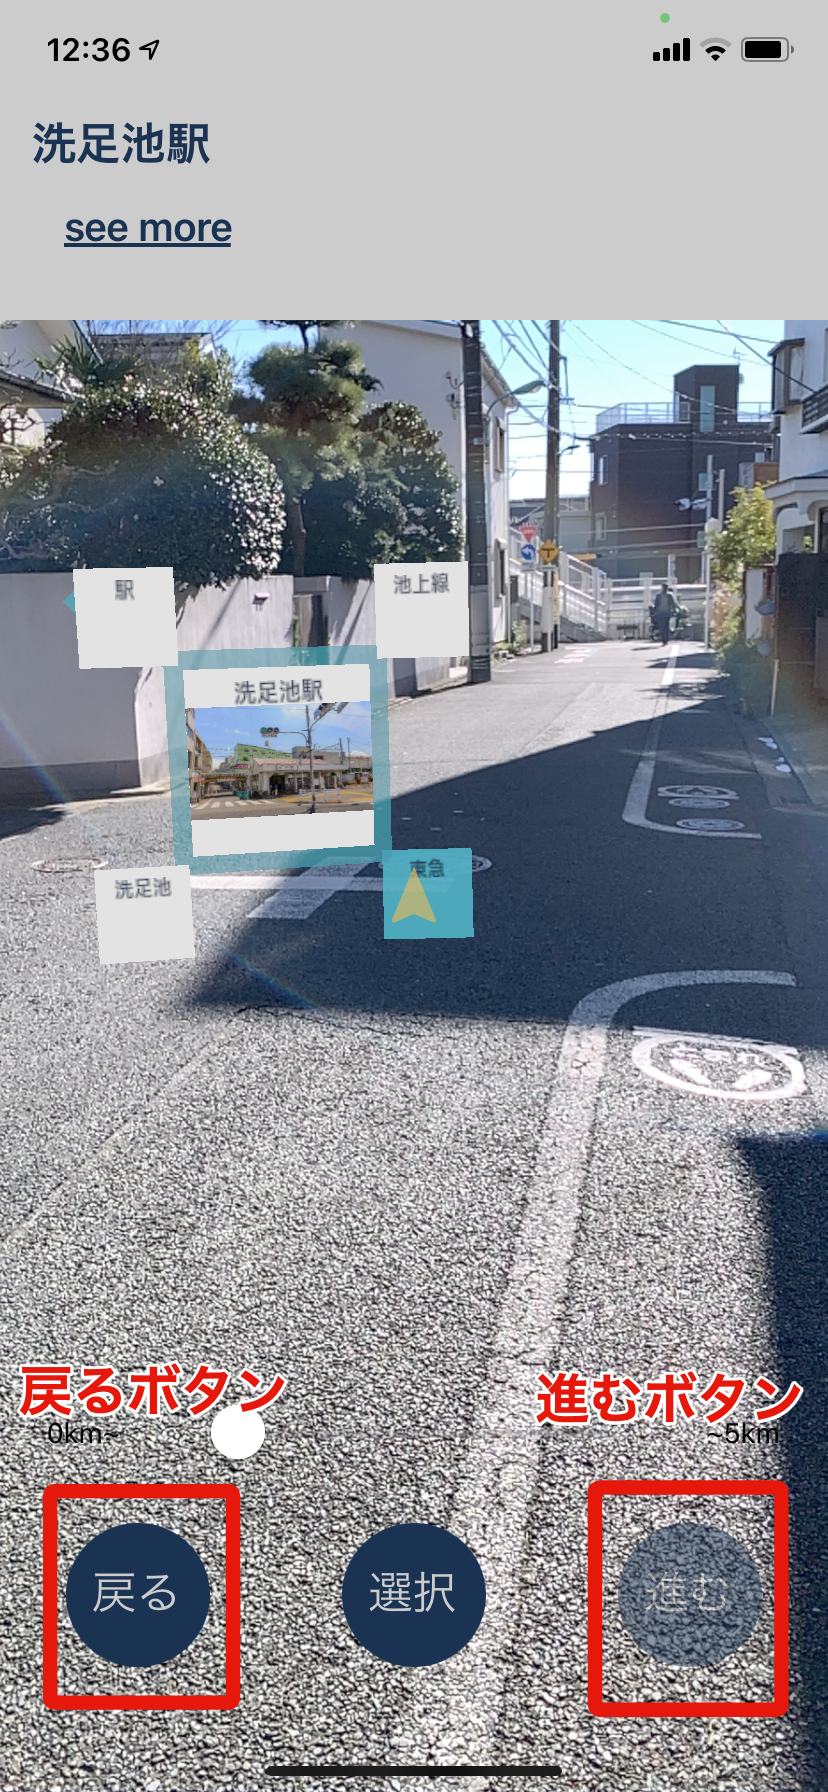
\includegraphics[height=100mm]{images/hypar_touch_history_button.png}
  \caption{進むボタンと戻るボタン} \label{fig:hypar_touch_history_button}
\end{figure}

\subsubsection{ScrapboxによるAR情報法の追加・編集}
HypAR Touchアプリに表示されるAR情報はNFCタグで指定されたScrapboxのプロジェクトをもとに生成される。
Scrapboxのプロジェクトにあるページのうち、Location記法によって位置情報の記述のあるページがアプリ側で表示されるAR情報と対応する。

\paragraph*{ARで表示する情報を追加する}
AR情報はScrapboxのページと対応しているため、新しくページを作成し、以下の2点の情報を記入することでAR情報が登録される。
\begin{itemize}
  \item ページタイトル
  
  図\ref{fig:scrapbox_ar_new}の\textcircled{\scriptsize{1}}部分であり、ページを作る上で必須となる項目である。
  このタイトルはHypAR Touchアプリ側でサムネイルとともにAR表示される。

  \item Location記法による記述
  
  Scrapboxにはソースコード \ref{google_map_url}のようなGoogle MapsのURLをソースコード \ref{location}のようなLocation記法に変換し、図\ref{fig:scrapbox_ar_new}の\textcircled{\scriptsize{2}}のようにマップとして表示する機能がある。
  この機能を利用し、AR情報を追加したい場所を中心としたGoogleMapのURLをScrapboxに貼り付けることでAR上で表示する場所を指定する。

  \begin{lstlisting}[caption=googleMapのURL, label=google_map_url]
    https://www.google.com/maps/place/%E6%9D%B1%E4%BA%AC%E9%A7%85/@35.681502,139.7671784,17z/data=!4m5!3m4!1s0x60188bfbd89f700b:0x277c49ba34ed38!8m2!3d35.6812362!4d139.7671248
  \end{lstlisting}

  \begin{lstlisting}[caption=Location記法, label=location]
    [N35.681502,E139.7671784,Z16 東京駅]
  \end{lstlisting}
\end{itemize}

\begin{figure}[H]
  \centering
  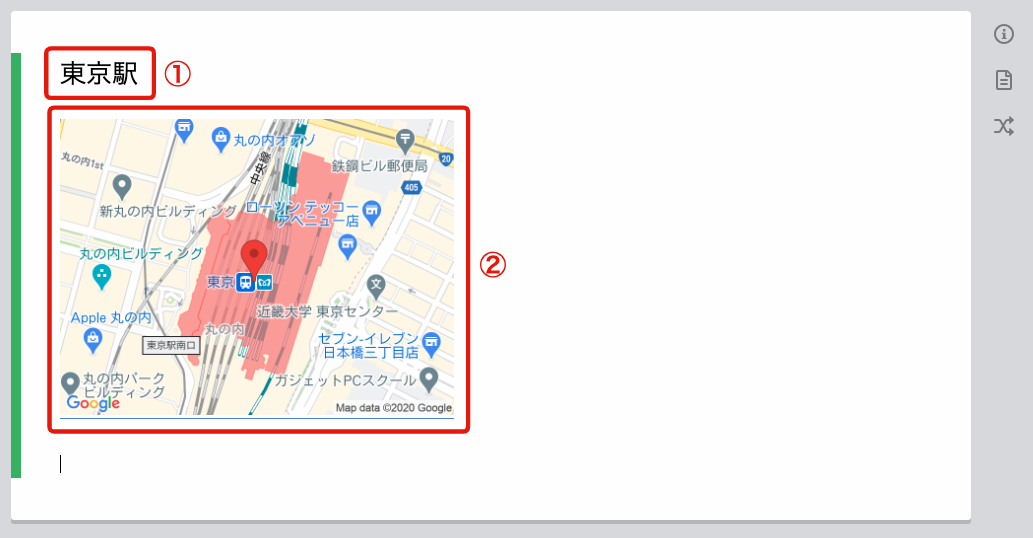
\includegraphics[width=120mm]{images/scrapbox_ar_new.png}
  \caption{新しくページを作成した時} \label{fig:scrapbox_ar_new}
\end{figure}

\paragraph*{サムネイルを追加する}
Scrapboxでは画像のURLを\texttt{[]}で囲う、または画像をドラッグ・アンド・ドロップすることで図\ref{fig:scrapbox_thumbnail}のようにページに画像を表示させることができる。
このようにScrapboxのページに画像を貼ると、ページの一番上にある画像がAR表示でのサムネイルになる。(図\ref{fig:scrapbox_thumbnail_and_ar})

\begin{figure}[H]
  \centering
  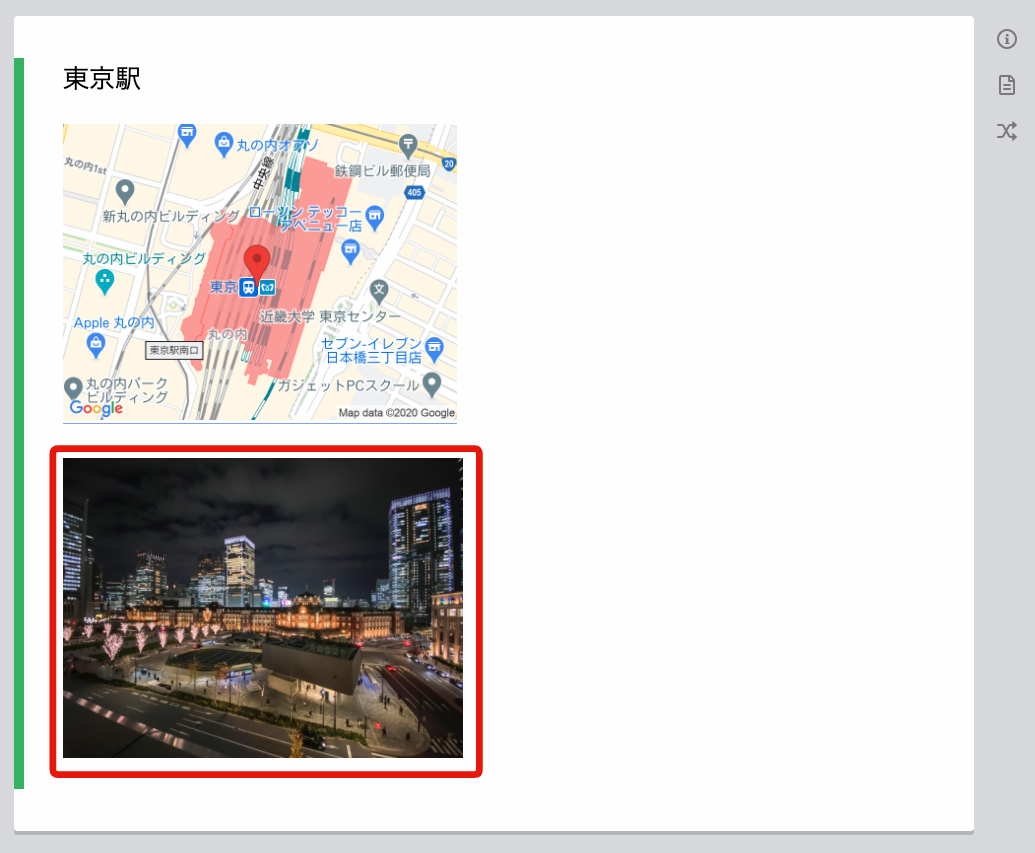
\includegraphics[width=120mm]{images/scrapbox_thumbnail.png}
  \caption{Scrapboxに貼り付けた画像} \label{fig:scrapbox_thumbnail}
\end{figure}

\begin{figure}[H]
  \centering
  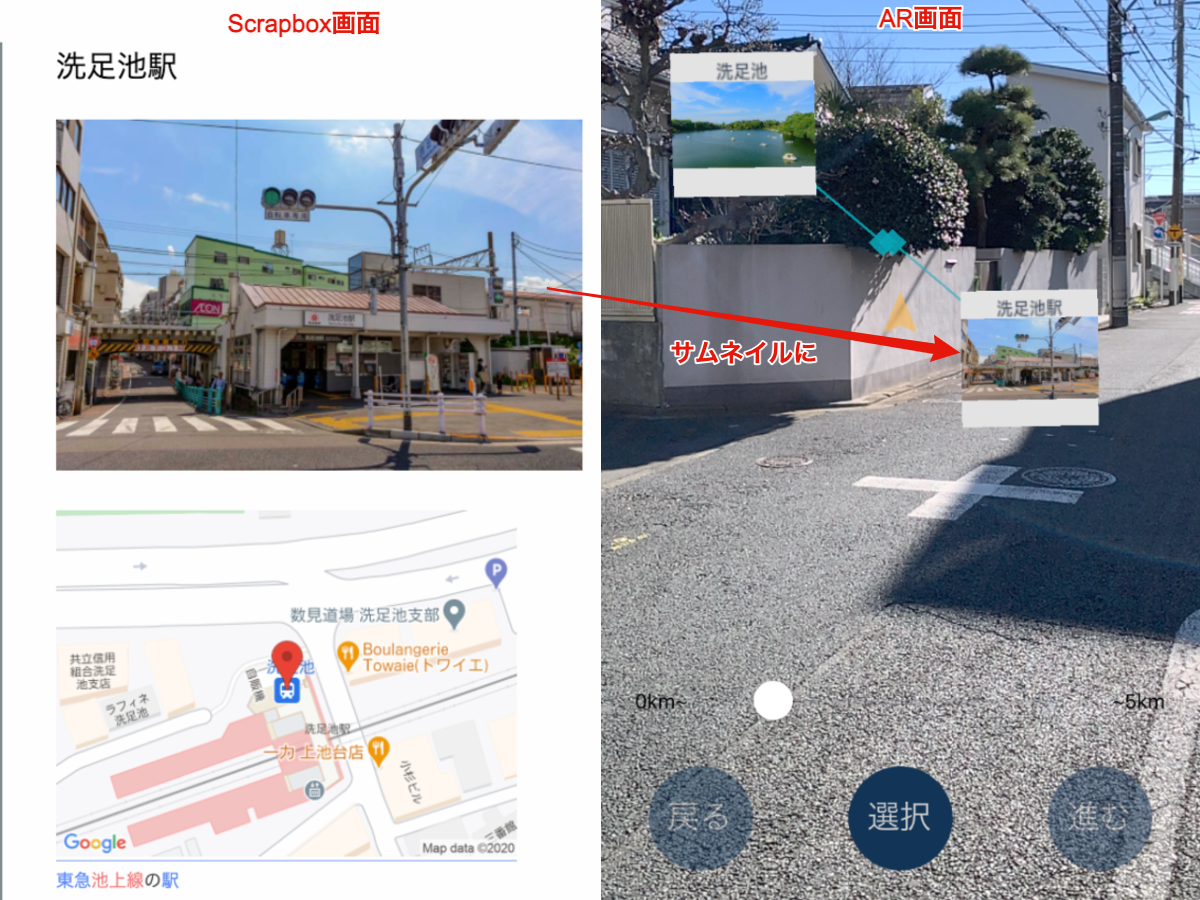
\includegraphics[width=120mm]{images/scrapbox_thumbnail_and_ar.png}
  \caption{Scrapbox上の画像とARでの表示} \label{fig:scrapbox_thumbnail_and_ar}
\end{figure}

\paragraph*{ハイパーリンクを利用して説明を書く}
Scrapboxでは単語を\texttt{[]}で囲うことにより同一Wiki内ページへのハイパーリンクとすることが可能である。
他ページヘのハイパーリンクが生成されるとAR上で関連情報として表示されるようになる(図\ref{fig:scrapbox_link_and_ar})。
ARで表示したい情報の説明を書き、説明文中の単語を積極的にハイパーリンクにすることで関連する情報を提示することができる。

\begin{figure}[H]
  \centering
  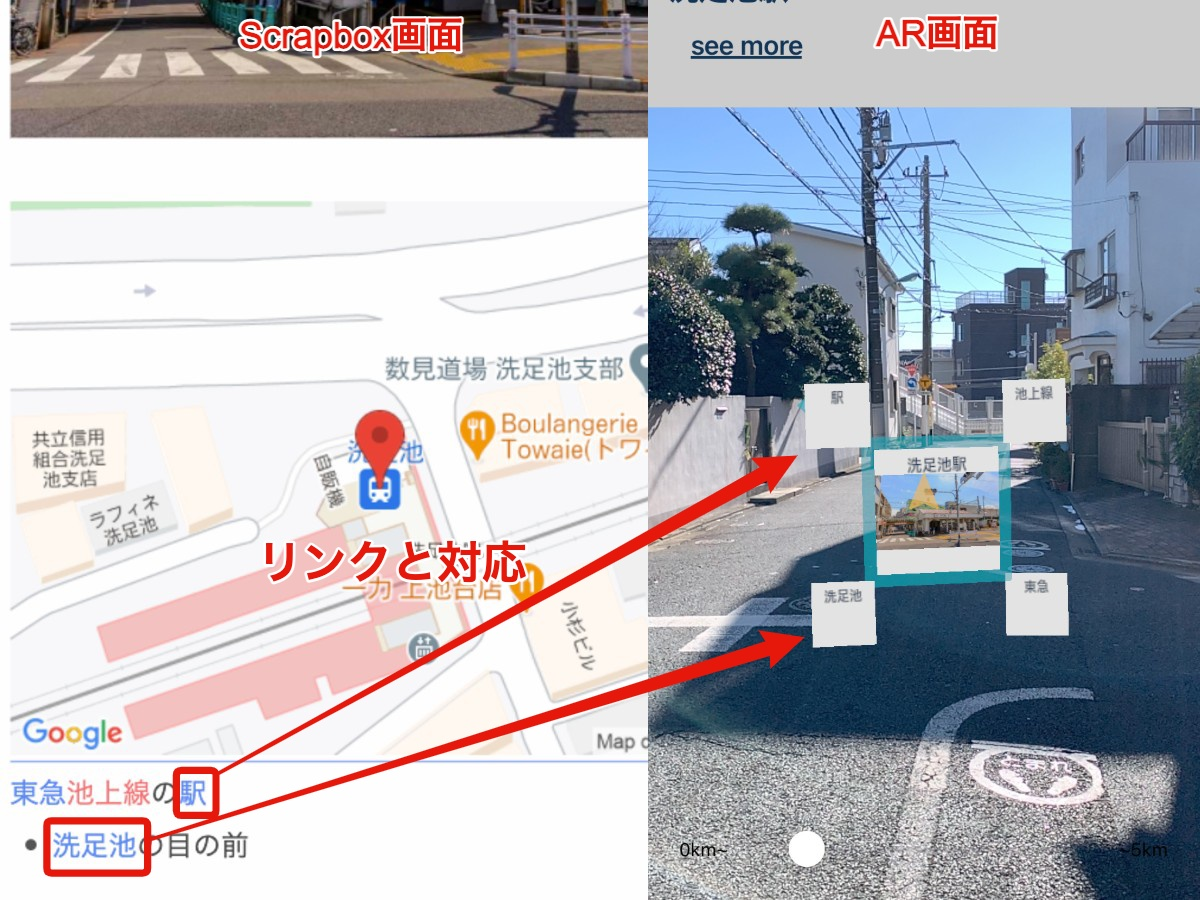
\includegraphics[width=120mm]{images/scrapbox_link_and_ar.jpg}
  \caption{Scrapbox上のリンクとARでの表示} \label{fig:scrapbox_link_and_ar}
\end{figure}

\subsubsection{NFCタグに対する情報の書き込み}
NFCタグにはISO/IEC 14443 TypeAに準拠したNTAGを利用する。
また情報を記録する際にはNFC FORUM\footnote{\textsf{https://nfc-forum.org}}によって標準化されているNDEFフォーマットで情報を書き込む。
書き込む情報は図\ref{fig:nfc_uri}のようにCustomURLSchemeに沿ったURIの形式で書き込む。

\begin{figure}[H]
  \centering
  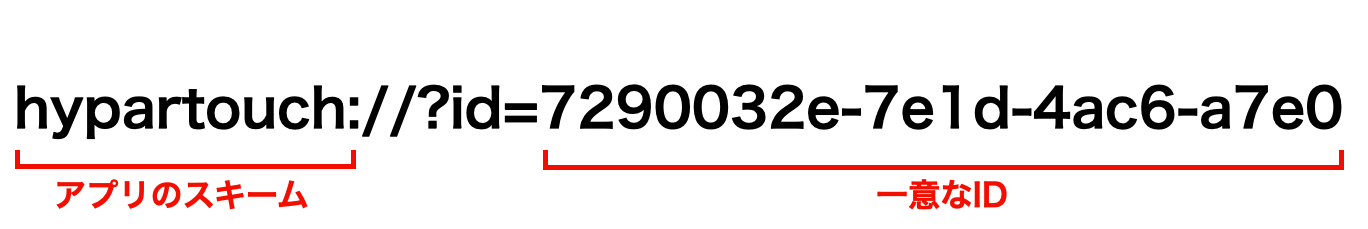
\includegraphics[width=120mm]{images/nfc_uri.png}
  \caption{NFCに書き込むURIデータ} \label{fig:nfc_uri}
\end{figure}

その上でタグに書き込んだIDと紐付ける形でHypAR Touchのサーバーに以下の情報を登録する。
\begin{itemize}
  \item 緯度経度
  \item タグの設置される向き(0〜360度)
  \item 表示するAR情報の元となるScrapboxのプロジェクト
  \item タッチした時に選択されているリンク情報
\end{itemize}
これらの情報はHypAR Touchアプリ内の登録画面(図\ref{fig:nfc_register_mobile})により登録可能である。

\begin{figure}[H]
  \centering
  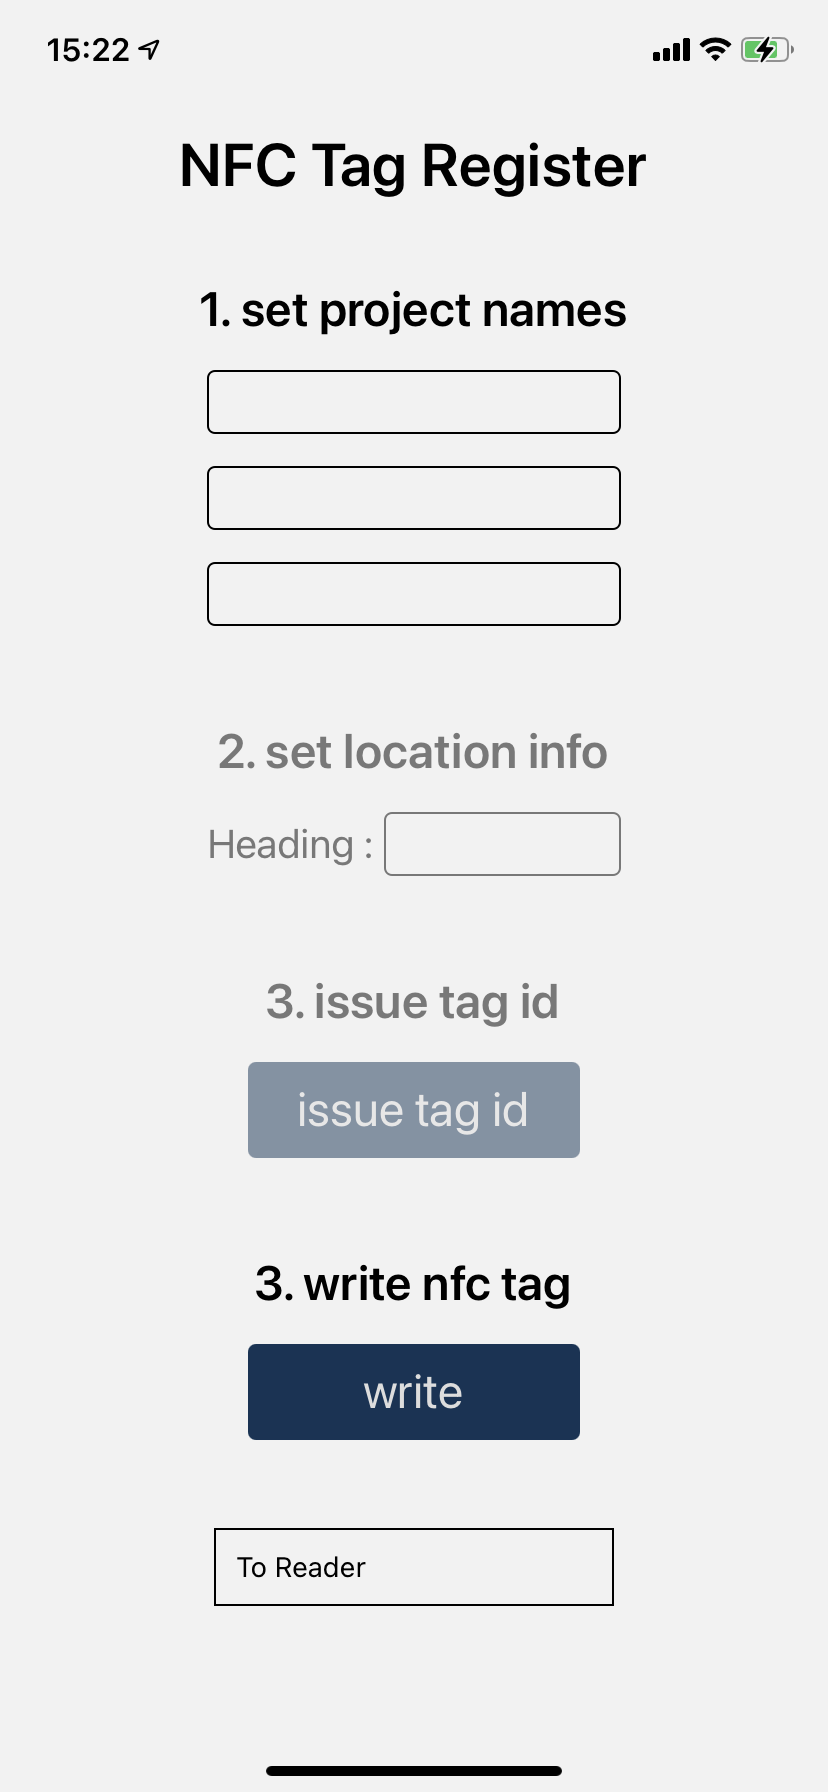
\includegraphics[height=100mm]{images/nfc_register_mobile.png}
  \caption{モバイルアプリでの登録} \label{fig:nfc_register_mobile}
\end{figure}
  % 本文4

\include{90_acknowledgment}  % 謝辞。要独自コマンド、include先参照のこと
\include{91_bibliography}  % 参考文献。要独自コマンド、include先参照のこと
\appendix
\include{92_appendix}    % 付録

\end{document}
